%package list
\documentclass{article}
\usepackage[top=3cm, bottom=3cm, outer=3cm, inner=3cm]{geometry}
\usepackage{multicol}
\usepackage{graphicx}
\usepackage{url}
%\usepackage{cite}
\usepackage{hyperref}
\usepackage{array}
%\usepackage{multicol}
\newcolumntype{x}[1]{>{\centering\arraybackslash\hspace{0pt}}p{#1}}
\usepackage{natbib}
\usepackage{pdfpages}
\usepackage{multirow}
\usepackage[normalem]{ulem}
\useunder{\uline}{\ul}{}
\usepackage{svg}
\usepackage{xcolor}
\usepackage{listings}
\lstdefinestyle{ascii-tree}{
    literate={├}{|}1 {─}{--}1 {└}{+}1 
  }
\lstset{basicstyle=\ttfamily,
  showstringspaces=false,
  commentstyle=\color{red},
  keywordstyle=\color{blue}
}
%\usepackage{booktabs}
\usepackage{caption}
\usepackage{subcaption}
\usepackage{float}
\usepackage{array}

\newcolumntype{M}[1]{>{\centering\arraybackslash}m{#1}}
\newcolumntype{N}{@{}m{0pt}@{}}


%%%%%%%%%%%%%%%%%%%%%%%%%%%%%%%%%%%%%%%%%%%%%%%%%%%%%%%%%%%%%%%%%%%%%%%%%%%%
%%%%%%%%%%%%%%%%%%%%%%%%%%%%%%%%%%%%%%%%%%%%%%%%%%%%%%%%%%%%%%%%%%%%%%%%%%%%
\newcommand{\itemEmail}{lluquecon@unsa.edu.pe fgarambel@unsa.edu.pe ajrahuacso@unsa.edu.pe wchoquehuancab@unsa.edu.pe}
\newcommand{\itemStudent}{Luis Guillermo Luque Condori, Fernando Miguel Garambel Marín, William Herderson Choquehuanca Berna, Jeans Anthony Ajra Huacso}
\newcommand{\itemCourse}{Laboratorio de P web}
\newcommand{\itemCourseCode}{20233478}
\newcommand{\itemSemester}{III}
\newcommand{\itemUniversity}{Universidad Nacional de San Agustín de Arequipa}
\newcommand{\itemFaculty}{Facultad de Ingeniería de Producción y Servicios}
\newcommand{\itemDepartment}{Departamento Académico de Ingeniería de Sistemas e Informática}
\newcommand{\itemSchool}{Escuela Profesional de Ingeniería de Sistemas}
\newcommand{\itemAcademic}{2024 - A}
\newcommand{\itemInput}{Del 09 de abril del 2024}
\newcommand{\itemOutput}{Al 18 de mayo del 2024}
\newcommand{\itemPracticeNumber}{04}
\newcommand{\itemTheme}{Ajax}
%%%%%%%%%%%%%%%%%%%%%%%%%%%%%%%%%%%%%%%%%%%%%%%%%%%%%%%%%%%%%%%%%%%%%%%%%%%%
%%%%%%%%%%%%%%%%%%%%%%%%%%%%%%%%%%%%%%%%%%%%%%%%%%%%%%%%%%%%%%%%%%%%%%%%%%%%

\usepackage[english,spanish]{babel}
\usepackage[utf8]{inputenc}
\AtBeginDocument{\selectlanguage{spanish}}
\renewcommand{\figurename}{Figura}
\renewcommand{\refname}{Referencias}
\renewcommand{\tablename}{Tabla} %esto no funciona cuando se usa babel
\AtBeginDocument{%
	\renewcommand\tablename{Tabla}
}

\usepackage{fancyhdr}
\pagestyle{fancy}
\fancyhf{}
\setlength{\headheight}{30pt}
\renewcommand{\headrulewidth}{1pt}
\renewcommand{\footrulewidth}{1pt}
\fancyhead[L]{\raisebox{-0.2\height}{
\includegraphics[width=3cm]{img/logo_episunsa.png}}}
\fancyhead[C]{\fontsize{7}{7}\selectfont	\itemUniversity \\ \itemFaculty \\ \itemDepartment \\ \itemSchool \\ \textbf{\itemCourse}}
\fancyhead[R]{\raisebox{-0.2\height}{
\includegraphics[width=1.2cm]{img/logo_abet}}}
\fancyfoot[L]{Estudiante Luis Luque Condori}
\fancyfoot[C]{\itemCourse}
\fancyfoot[R]{Página \thepage}

% para el codigo fuente
\usepackage{listings}
\usepackage{color, colortbl}
\definecolor{dkgreen}{rgb}{0,0.6,0}
\definecolor{gray}{rgb}{0.5,0.5,0.5}
\definecolor{mauve}{rgb}{0.58,0,0.82}
\definecolor{codebackground}{rgb}{0.95, 0.95, 0.92}
\definecolor{tablebackground}{rgb}{0.8, 0, 0}

\lstset{frame=tb,
	language=bash,
	aboveskip=3mm,
	belowskip=3mm,
	showstringspaces=false,
	columns=flexible,
	basicstyle={\small\ttfamily},
	numbers=none,
	numberstyle=\tiny\color{gray},
	keywordstyle=\color{blue},
	commentstyle=\color{dkgreen},
	stringstyle=\color{mauve},
	breaklines=true,
	breakatwhitespace=true,
	tabsize=3,
	backgroundcolor= \color{codebackground},
}

\begin{document}
	
	\vspace*{10px}
	
	\begin{center}	
		\fontsize{17}{17} \textbf{ Informe de Laboratorio \itemPracticeNumber}
	\end{center}
	\centerline{\textbf{\Large Tema: \itemTheme}}
	%\vspace*{0.5cm}	

	\begin{flushright}
		\begin{tabular}{|M{2.5cm}|N|}
			\hline 
			\rowcolor{tablebackground}
			\color{white} \textbf{Nota}  \\
			\hline 
			     \\[30pt]
			\hline 			
		\end{tabular}
	\end{flushright}	

	\begin{table}[H]
		\begin{tabular}{|x{4.7cm}|x{4.8cm}|x{4.8cm}|}
			\hline 
			\rowcolor{tablebackground}
			\color{white} \textbf{Estudiante} & \color{white}\textbf{Escuela}  & \color{white}\textbf{Asignatura}   \\
			\hline 
			{\itemStudent \par \itemEmail} & \itemSchool & {\itemCourse \par Semestre: \itemSemester \par Código: \itemCourseCode}     \\
			\hline 			
		\end{tabular}
	\end{table}		
	
	\begin{table}[H]
		\begin{tabular}{|x{4.7cm}|x{4.8cm}|x{4.8cm}|}
			\hline 
			\rowcolor{tablebackground}
			\color{white}\textbf{Laboratorio} & \color{white}\textbf{Tema}  & \color{white}\textbf{Duración}   \\
			\hline 
			\itemPracticeNumber & \itemTheme & 04 horas   \\
			\hline 
		\end{tabular}
	\end{table}
	
	\begin{table}[H]
		\begin{tabular}{|x{4.7cm}|x{4.8cm}|x{4.8cm}|}
			\hline 
			\rowcolor{tablebackground}
			\color{white}\textbf{Semestre académico} & \color{white}\textbf{Fecha de inicio}  & \color{white}\textbf{Fecha de entrega}   \\
			\hline 
			\itemAcademic & \itemInput &  \itemOutput  \\
			\hline 
		\end{tabular}
	\end{table}

	\clearpage




	\section{Tarea Documento}
	\begin{itemize}		
		\item Listar los archivos Markdown disponibles
		\item Ver el contenido de un archivo Markdown traducido a HTML
		\item Crear nuevos archivos MarkDown y almacenarlos en el servidor
	\end{itemize}
	\section{Tarea Plataforma}
	\begin{itemize}		
		\item Liste todas las “regiones”
		\item Muestre el número total de confirmados por región
		\item Encuentre las 10 regiones cuya suma total sea la mayor
		\item Visualice un gráfico en el tiempo de los valores para la región de Arequipa
		\item Haga gráficos comparativos entre regiones usando líneas
		\item Visualice un gráfico comparativo del crecimiento en regiones excepto Lima y Callao
		\item Haga gráficos comparativos entre regiones elegidas por el usuario.
		\item Visualice un gráfico comparativo del crecimiento en regiones excepto Lima y Callao, mostrando el número de confirmados por cada día
	\end{itemize}
	\section{URL GitHub}
	\begin{itemize}
		\item \url{https://github.com/FernandoGarambelM/Ajax.git}
	\end{itemize}
	\section{Tareas Documento}
	\subsection{Listar los archivos Markdown disponibles}
	\subsection{Ver el contenido de un archivo Markdown traducido a HTML}
	\subsection{Crear nuevos archivos MarkDown y almacenarlos en el servidor}


	\clearpage

	\section{Tareas Plataforma}
	\subsection{Liste las regiones}
	\begin{itemize}
		\item HTML
		\begin{figure}[H]
			\centering
			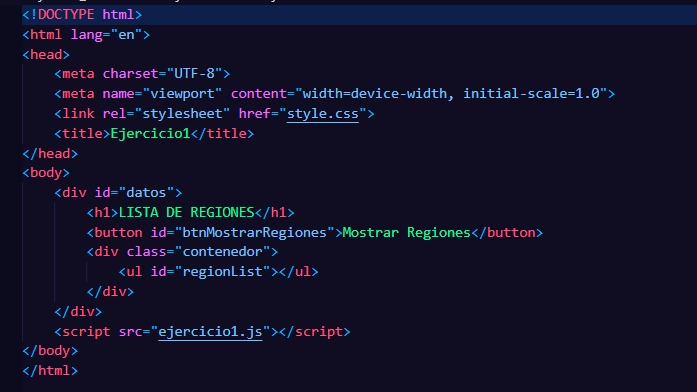
\includegraphics[width=1.0\textwidth,keepaspectratio]{img/Ejer1T2HTML.jpg}
			%\includesvg{img/automata.svg}
			%\label{img:mot2}
			%\caption{Product backlog.}
		\end{figure}
		\item Script
		\begin{figure}[H]
			\centering
			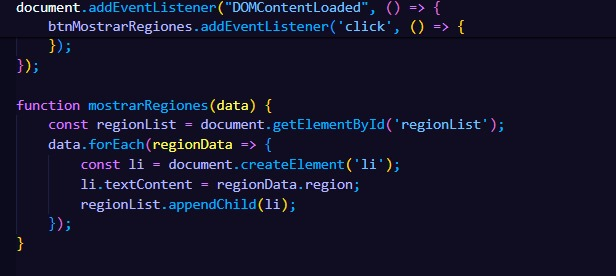
\includegraphics[width=1.0\textwidth,keepaspectratio]{img/Ejer1T2Script.jpg}
			%\includesvg{img/automata.svg}
			%\label{img:mot2}
			%\caption{Product backlog.}
		\end{figure}
		\item Página
		\begin{figure}[H]
			\centering
			\includegraphics[width=1.0\textwidth,keepaspectratio]{img/Ejer1T2Página.jpg}
			%\includesvg{img/automata.svg}
			%\label{img:mot2}
			%\caption{Product backlog.}
		\end{figure}
		\item Resultado
		\begin{figure}[H]
			\centering
			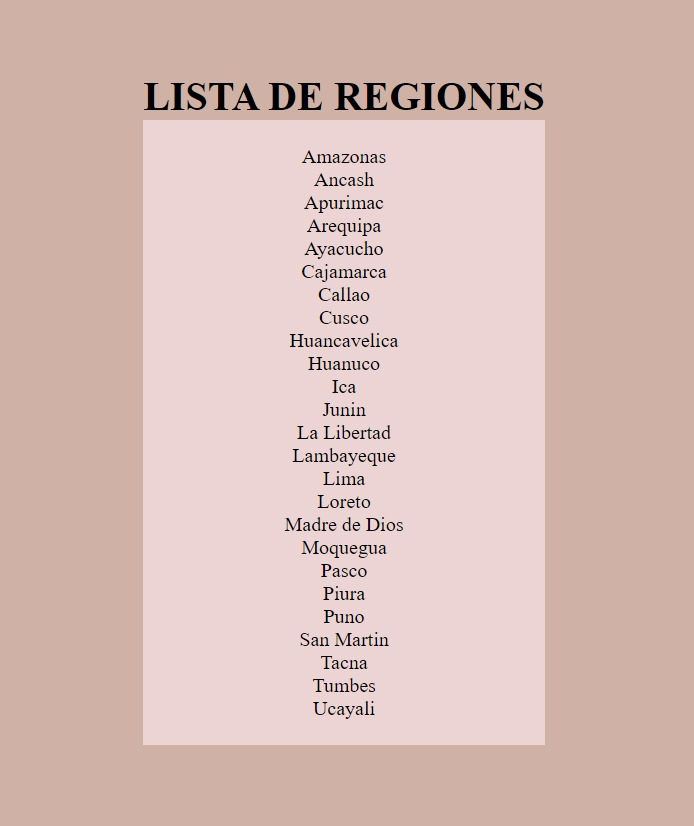
\includegraphics[width=1.0\textwidth,keepaspectratio]{img/Ejer1T2result.jpg}
			%\includesvg{img/automata.svg}
			%\label{img:mot2}
			%\caption{Product backlog.}
		\end{figure}
	\end{itemize}

	\subsection{Muestre el número total de confirmados por región}
	\begin{itemize}
		\item HTML
		\begin{figure}[H]
			\centering
			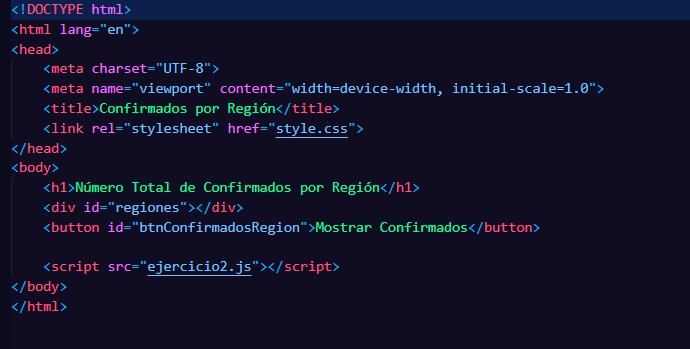
\includegraphics[width=1.0\textwidth,keepaspectratio]{img/Ejer2T2HTML.jpg}
			%\includesvg{img/automata.svg}
			%\label{img:mot2}
			%\caption{Product backlog.}
		\end{figure}
		\item Script
		\begin{figure}[H]
			\centering
			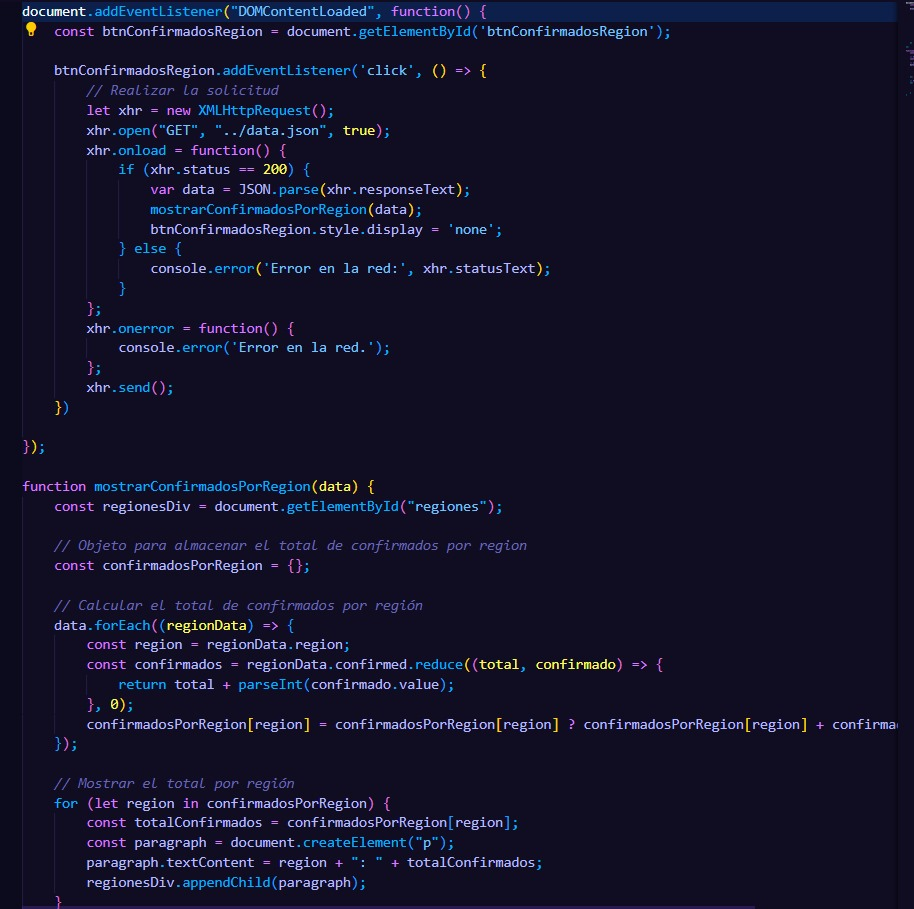
\includegraphics[width=1.0\textwidth,keepaspectratio]{img/Ejer2T2Script.jpg}
			%\includesvg{img/automata.svg}
			%\label{img:mot2}
			%\caption{Product backlog.}
		\end{figure}
		\item Página
		\begin{figure}[H]
			\centering
			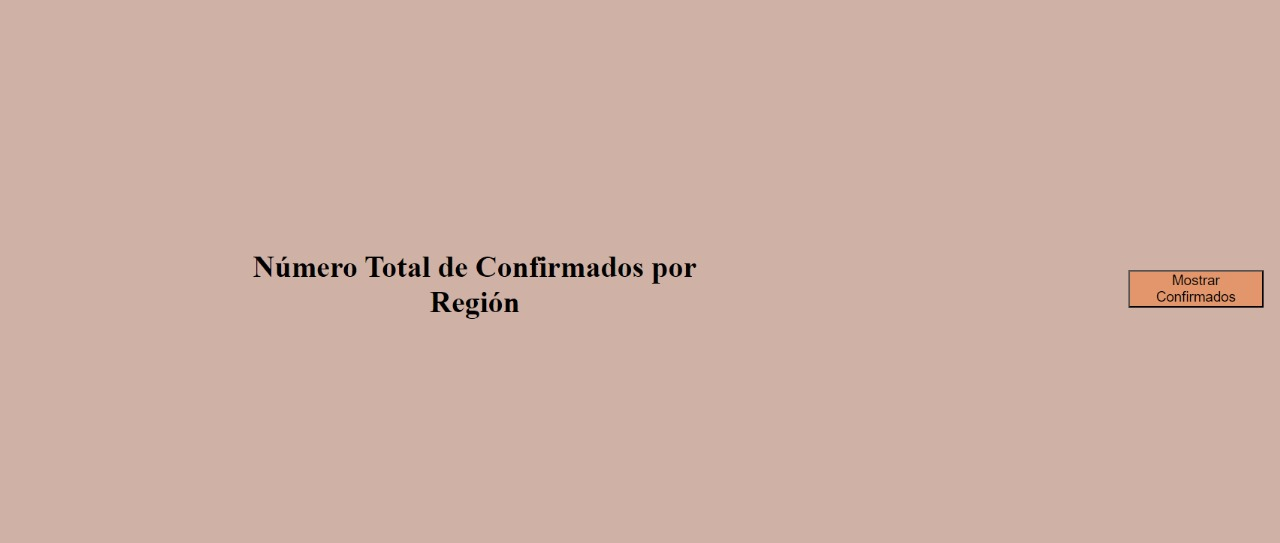
\includegraphics[width=1.0\textwidth,keepaspectratio]{img/Ejer2T2Pagina.jpg}
			%\includesvg{img/automata.svg}
			%\label{img:mot2}
			%\caption{Product backlog.}
		\end{figure}
		\item Resultado
		\begin{figure}[H]
			\centering
			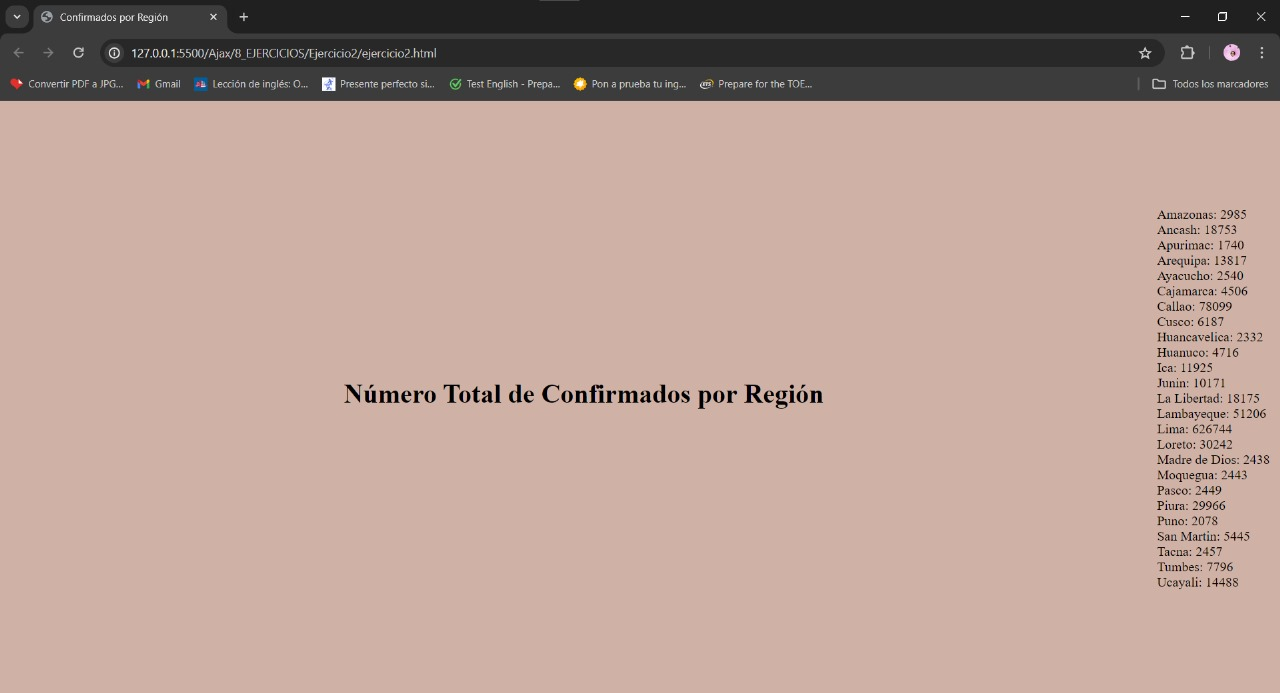
\includegraphics[width=1.0\textwidth,keepaspectratio]{img/Ejer2T2Result.jpg}
			%\includesvg{img/automata.svg}
			%\label{img:mot2}
			%\caption{Product backlog.}
		\end{figure}
	\end{itemize}

	\subsection{Encuentre las 10 regiones cuya suma total sea la mayor}

	\begin{itemize}
		\item HTML
		\begin{figure}[H]
			\centering
			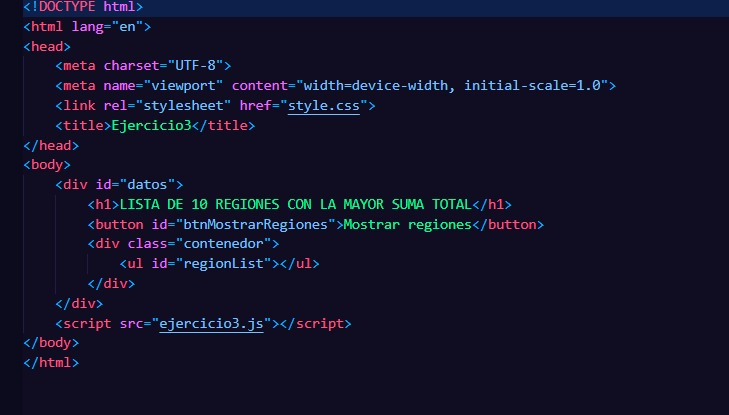
\includegraphics[width=1.0\textwidth,keepaspectratio]{img/Ejer3T2HTML.jpg}
			%\includesvg{img/automata.svg}
			%\label{img:mot2}
			%\caption{Product backlog.}
		\end{figure}
		\item Script
		\begin{figure}[H]
			\centering
			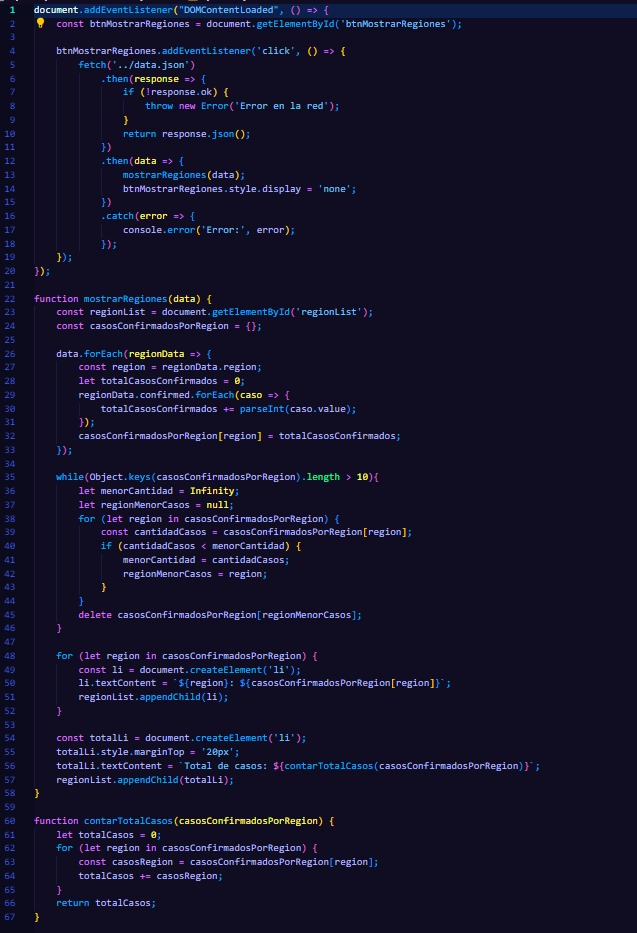
\includegraphics[width=1.0\textwidth,keepaspectratio]{img/Ejer3T2Script.jpg}
			%\includesvg{img/automata.svg}
			%\label{img:mot2}
			%\caption{Product backlog.}
		\end{figure}
		\item Página
		\begin{figure}[H]
			\centering
			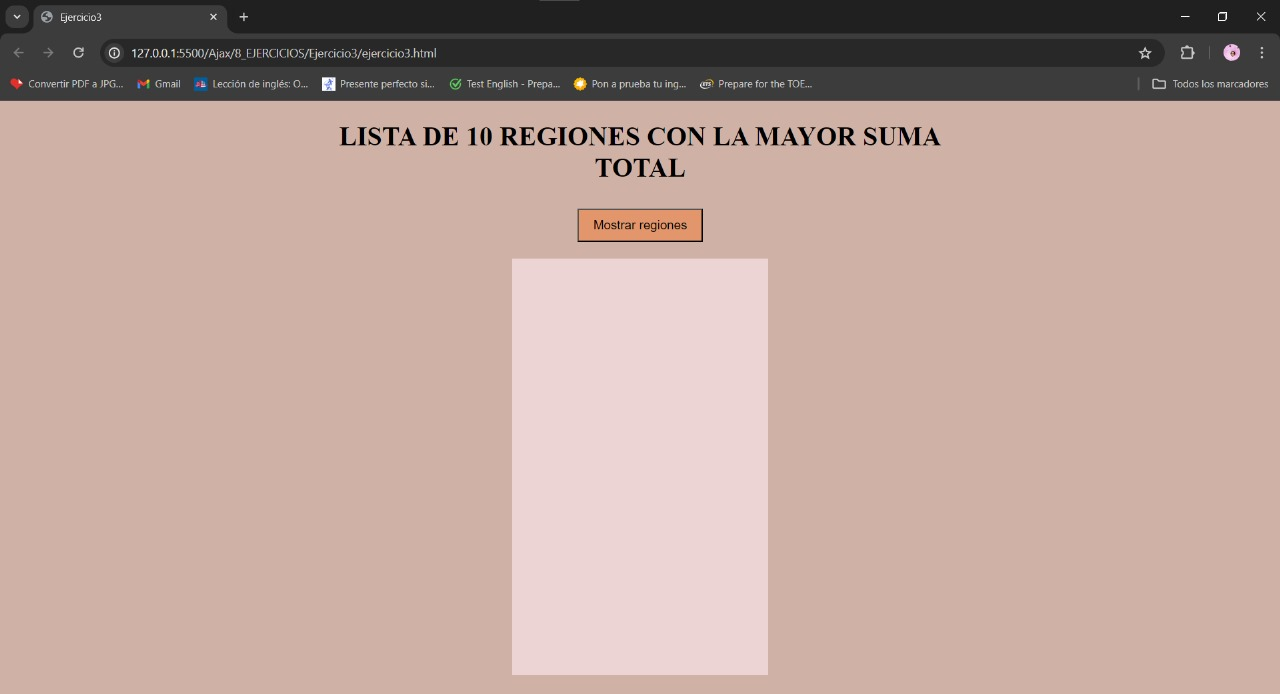
\includegraphics[width=1.0\textwidth,keepaspectratio]{img/Ejer3T2Pagina.jpg}
			%\includesvg{img/automata.svg}
			%\label{img:mot2}
			%\caption{Product backlog.}
		\end{figure}
		\item Resultado
		\begin{figure}[H]
			\centering
			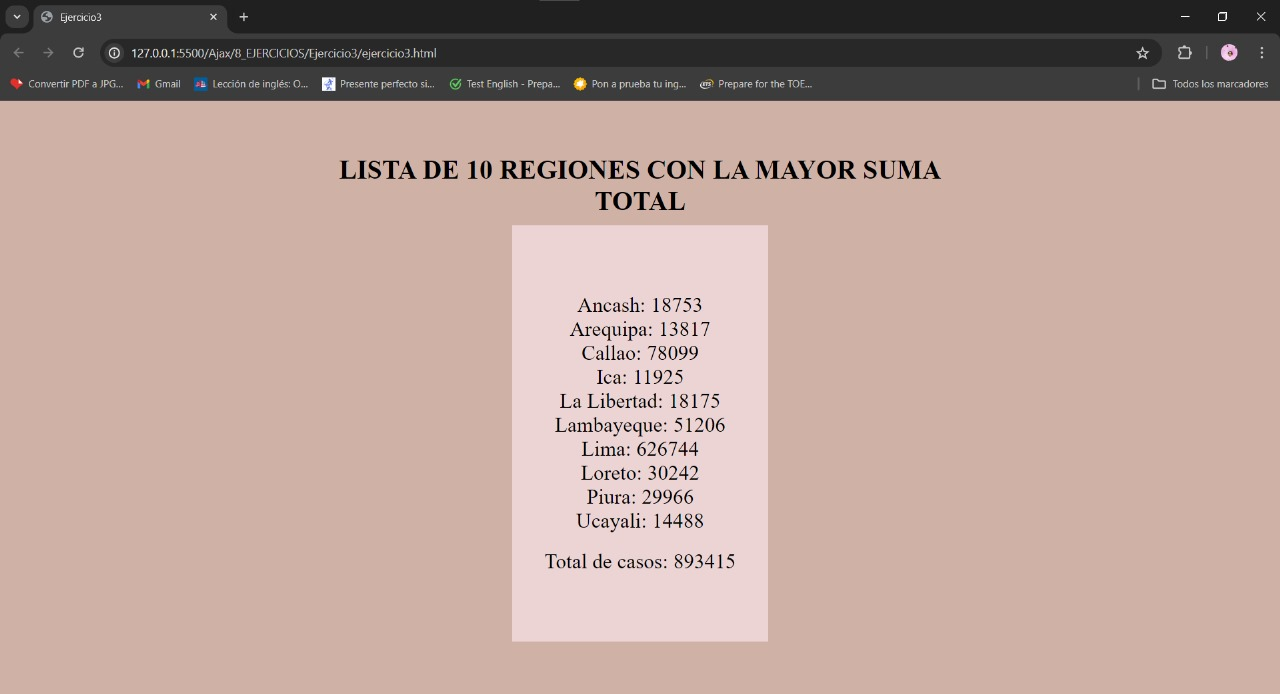
\includegraphics[width=1.0\textwidth,keepaspectratio]{img/Ejer3T2Result.jpg}
			%\includesvg{img/automata.svg}
			%\label{img:mot2}
			%\caption{Product backlog.}
		\end{figure}
	\end{itemize}

	\subsection{Visualice un gráfico en el tiempo de los valores para la región de Arequipa}
	
	\begin{itemize}
		\item HTML
		\begin{figure}[H]
			\centering
			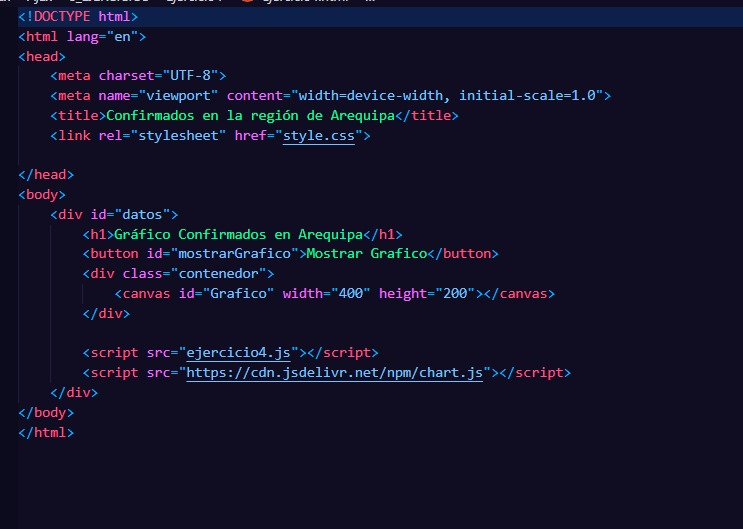
\includegraphics[width=1.0\textwidth,keepaspectratio]{img/Ejer4T2HTML.jpg}
			%\includesvg{img/automata.svg}
			%\label{img:mot2}
			%\caption{Product backlog.}
		\end{figure}
		\item Script
		\begin{figure}[H]
			\centering
			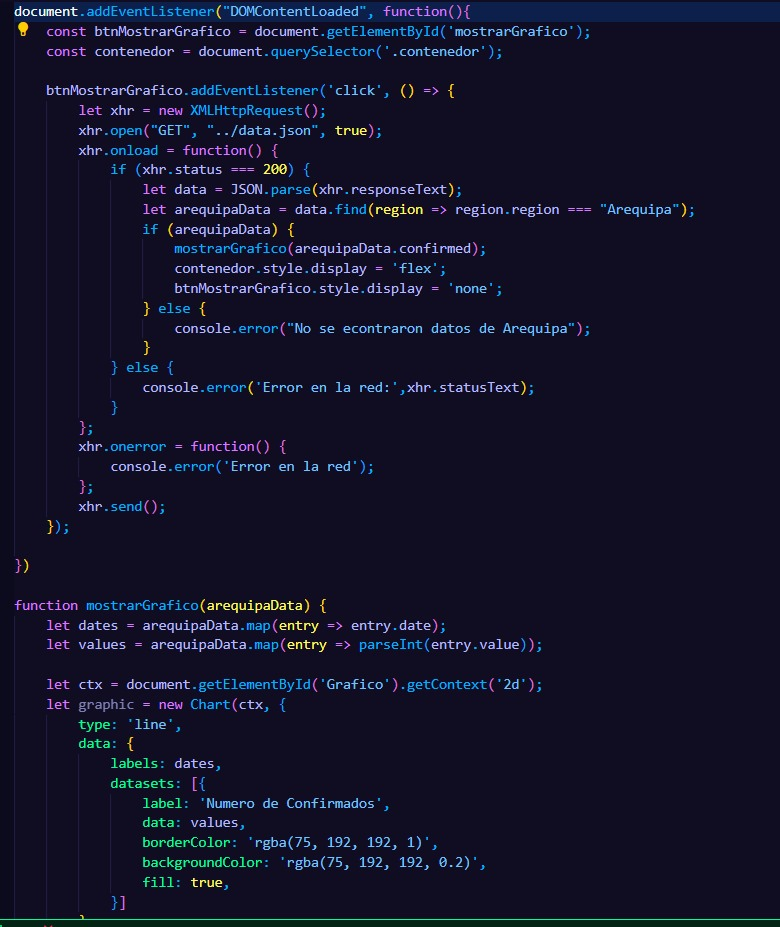
\includegraphics[width=1.0\textwidth,keepaspectratio]{img/Ejer4T2Script.jpg}
			%\includesvg{img/automata.svg}
			%\label{img:mot2}
			%\caption{Product backlog.}
		\end{figure}
		\item Página
		\begin{figure}[H]
			\centering
			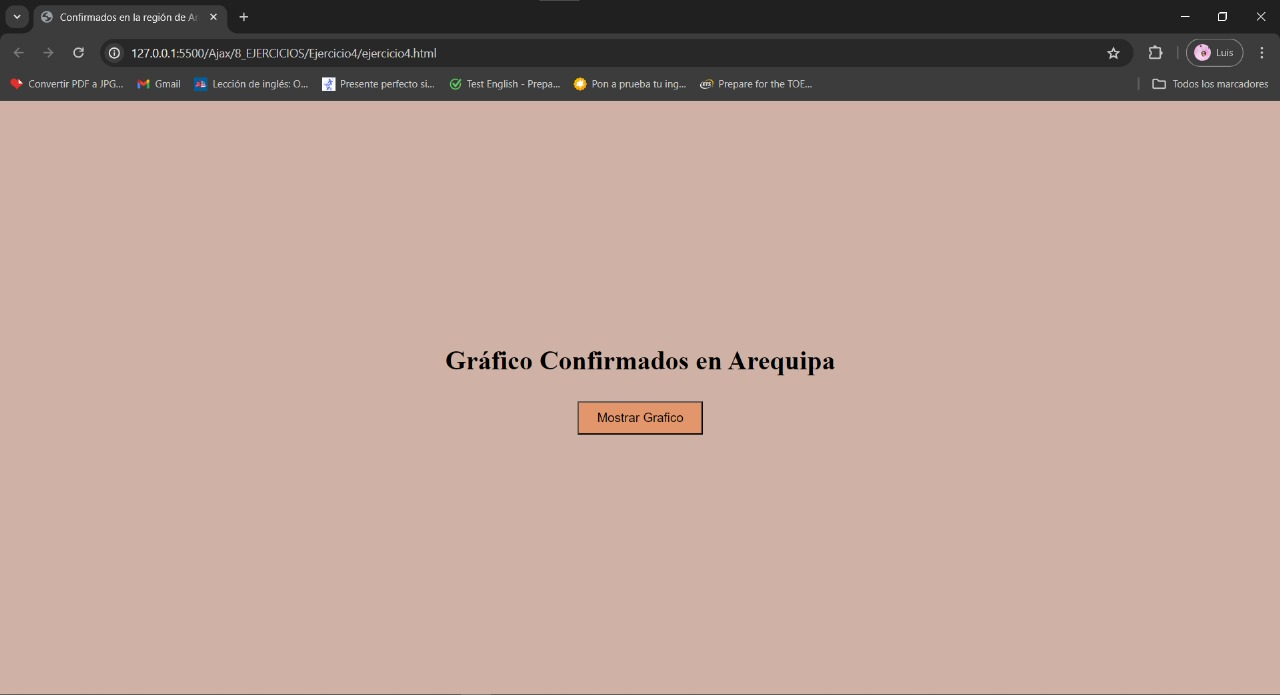
\includegraphics[width=1.0\textwidth,keepaspectratio]{img/Ejer4T2Pagina.jpg}
			%\includesvg{img/automata.svg}
			%\label{img:mot2}
			%\caption{Product backlog.}
		\end{figure}
		\item Resultado
		\begin{figure}[H]
			\centering
			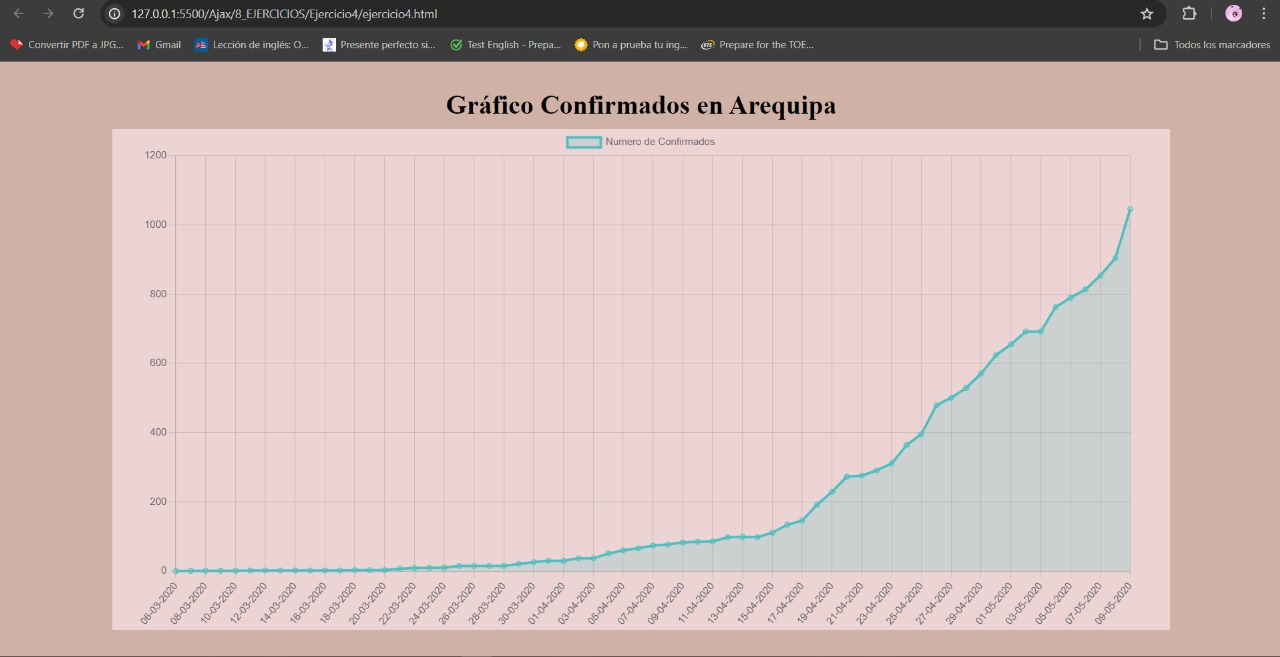
\includegraphics[width=1.0\textwidth,keepaspectratio]{img/Ejer4T2Result.jpg}
			%\includesvg{img/automata.svg}
			%\label{img:mot2}
			%\caption{Product backlog.}
		\end{figure}
	\end{itemize}
	
	\subsection{Haga gráficos comparativos entre regiones usando líneas}
	
	\begin{itemize}
		\item HTML
		\begin{figure}[H]
			\centering
			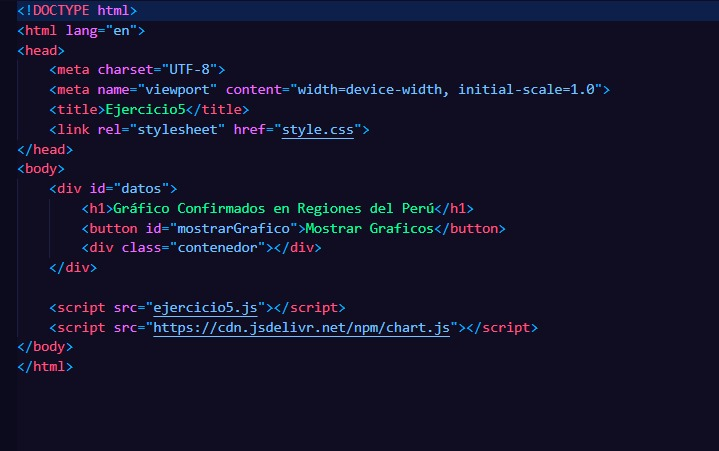
\includegraphics[width=1.0\textwidth,keepaspectratio]{img/Ejer5T2HTML.jpg}
			%\includesvg{img/automata.svg}
			%\label{img:mot2}
			%\caption{Product backlog.}
		\end{figure}
		\item Script
		\begin{figure}[H]
			\centering
			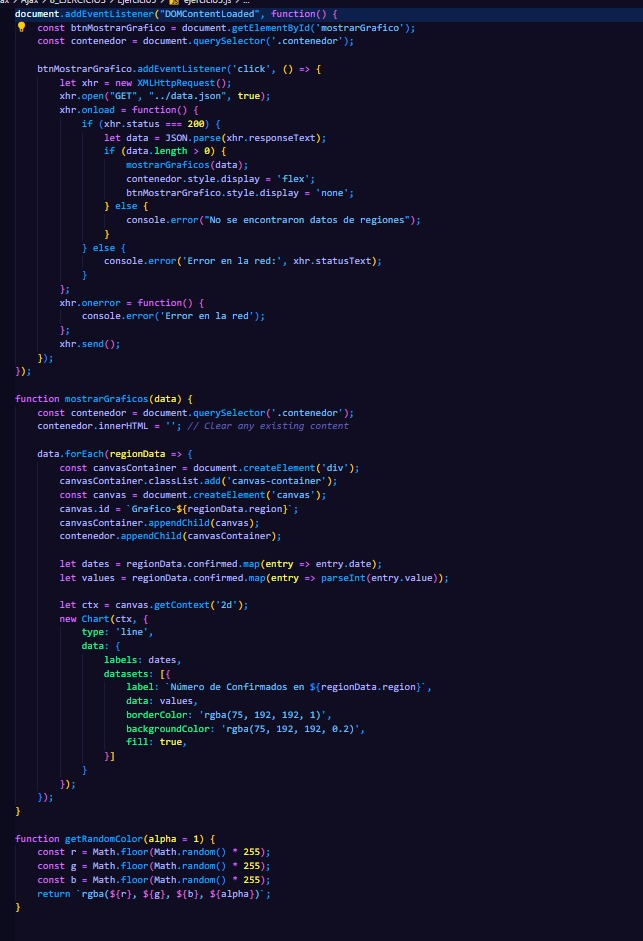
\includegraphics[width=1.0\textwidth,keepaspectratio]{img/Ejer5T2Sript.jpg}
			%\includesvg{img/automata.svg}
			%\label{img:mot2}
			%\caption{Product backlog.}
		\end{figure}
		\item Página
		\begin{figure}[H]
			\centering
			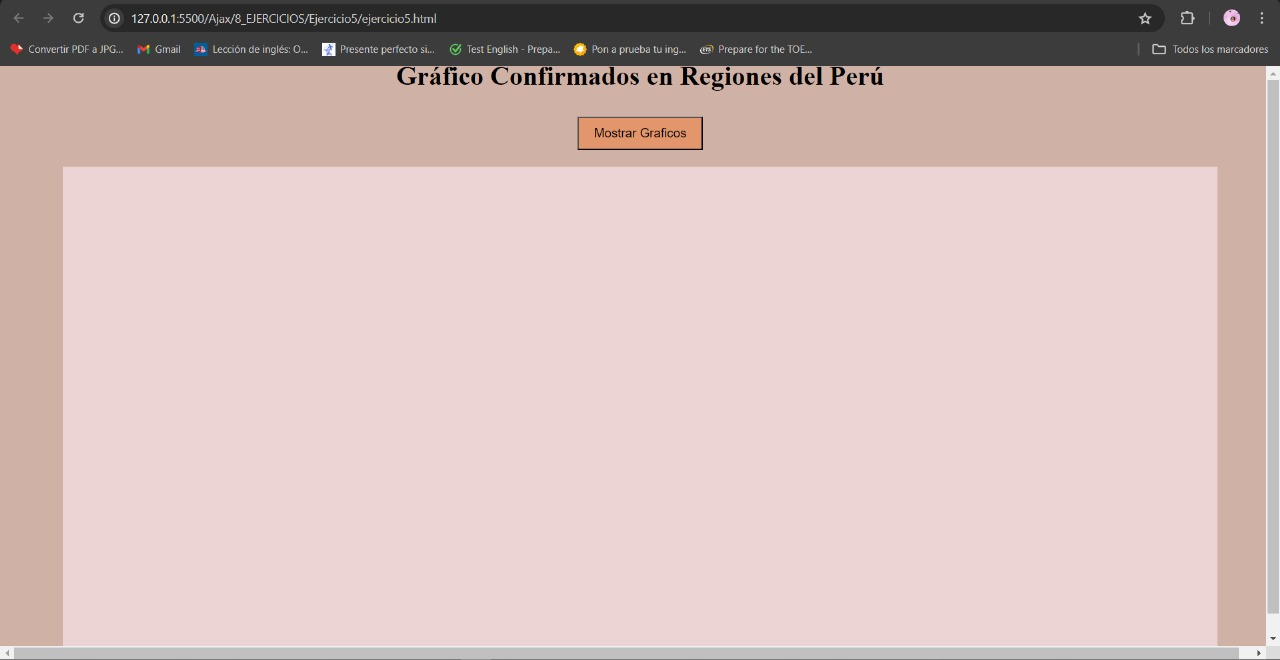
\includegraphics[width=1.0\textwidth,keepaspectratio]{img/Ejer5T2Pagina.jpg}
			%\includesvg{img/automata.svg}
			%\label{img:mot2}
			%\caption{Product backlog.}
		\end{figure}
		\item Resultado
		\begin{figure}[H]
			\centering
			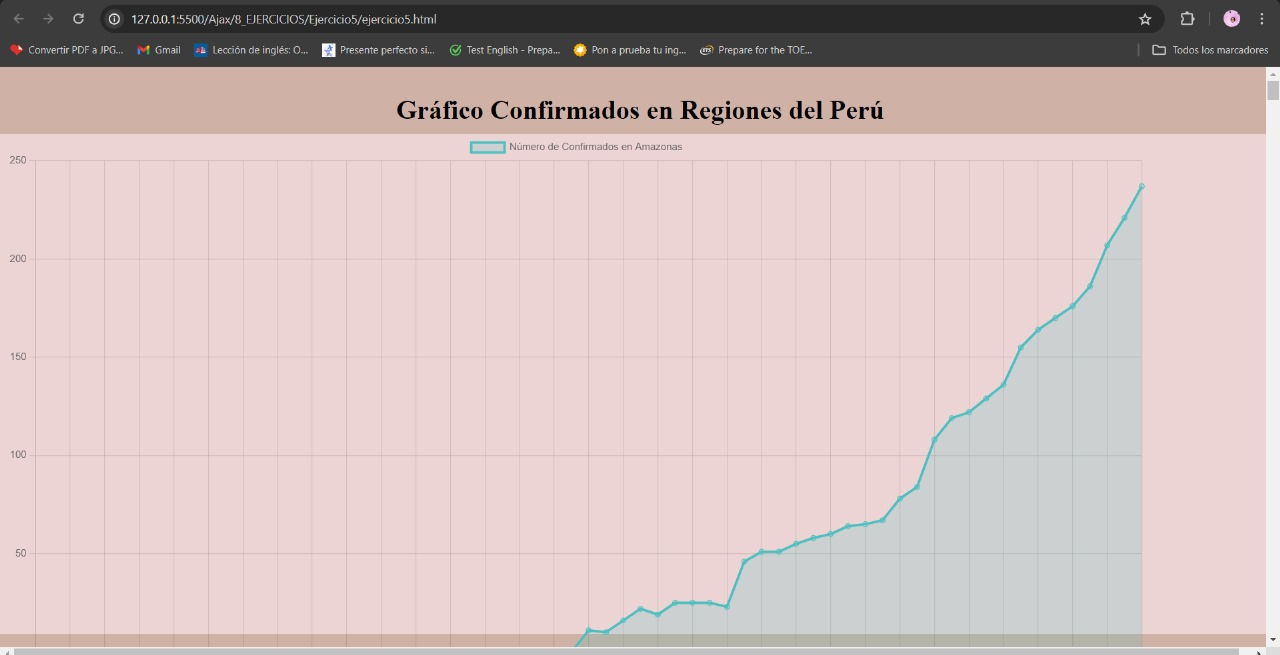
\includegraphics[width=1.0\textwidth,keepaspectratio]{img/Ejer5T2Result.jpg}
			%\includesvg{img/automata.svg}
			%\label{img:mot2}
			%\caption{Product backlog.}
		\end{figure}
	\end{itemize}
	
	\subsection{Visualice un gráfico comparativo del crecimiento en regiones excepto Lima y Callao}
	
	\begin{itemize}
		\item HTML
		\begin{figure}[H]
			\centering
			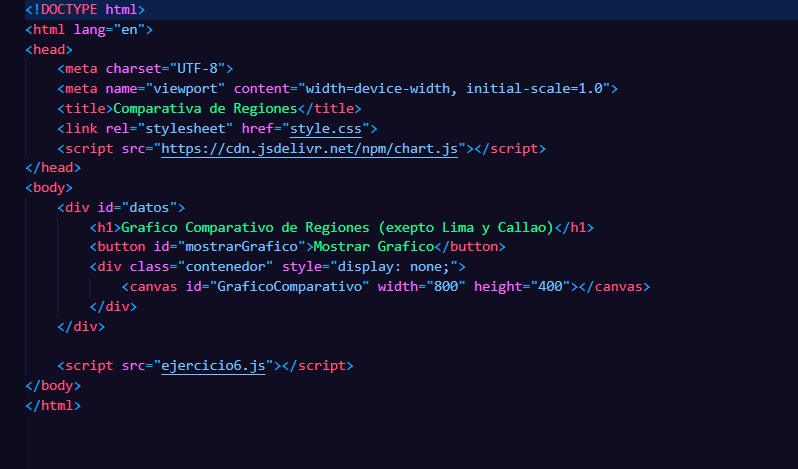
\includegraphics[width=1.0\textwidth,keepaspectratio]{img/Ejer6T2HTML.jpg}
			%\includesvg{img/automata.svg}
			%\label{img:mot2}
			%\caption{Product backlog.}
		\end{figure}
		\item Script
		\begin{figure}[H]
			\centering
			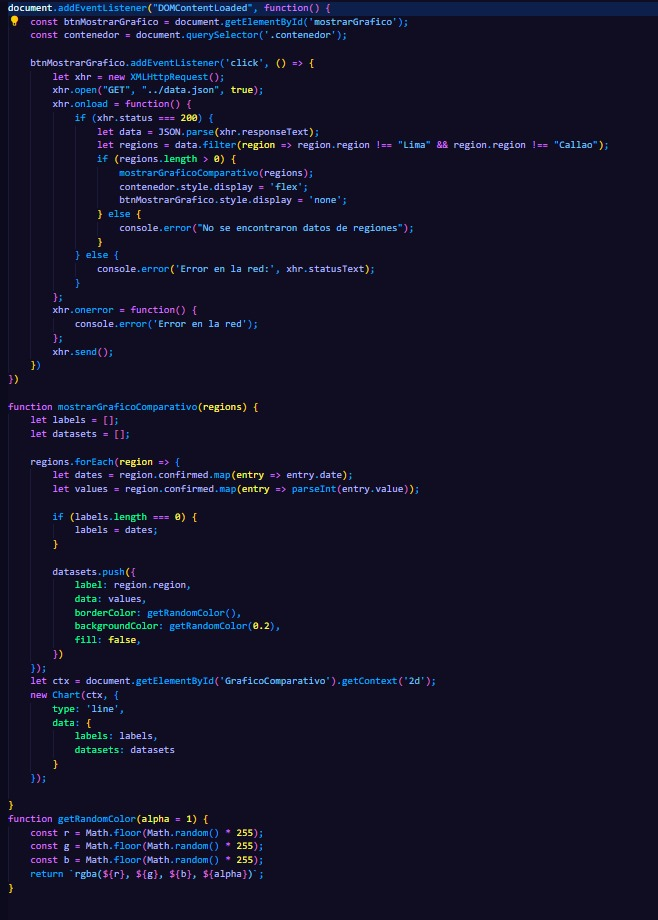
\includegraphics[width=1.0\textwidth,keepaspectratio]{img/Ejer6T2Scipr.jpg}
			%\includesvg{img/automata.svg}
			%\label{img:mot2}
			%\caption{Product backlog.}
		\end{figure}
		\item Página
		\begin{figure}[H]
			\centering
			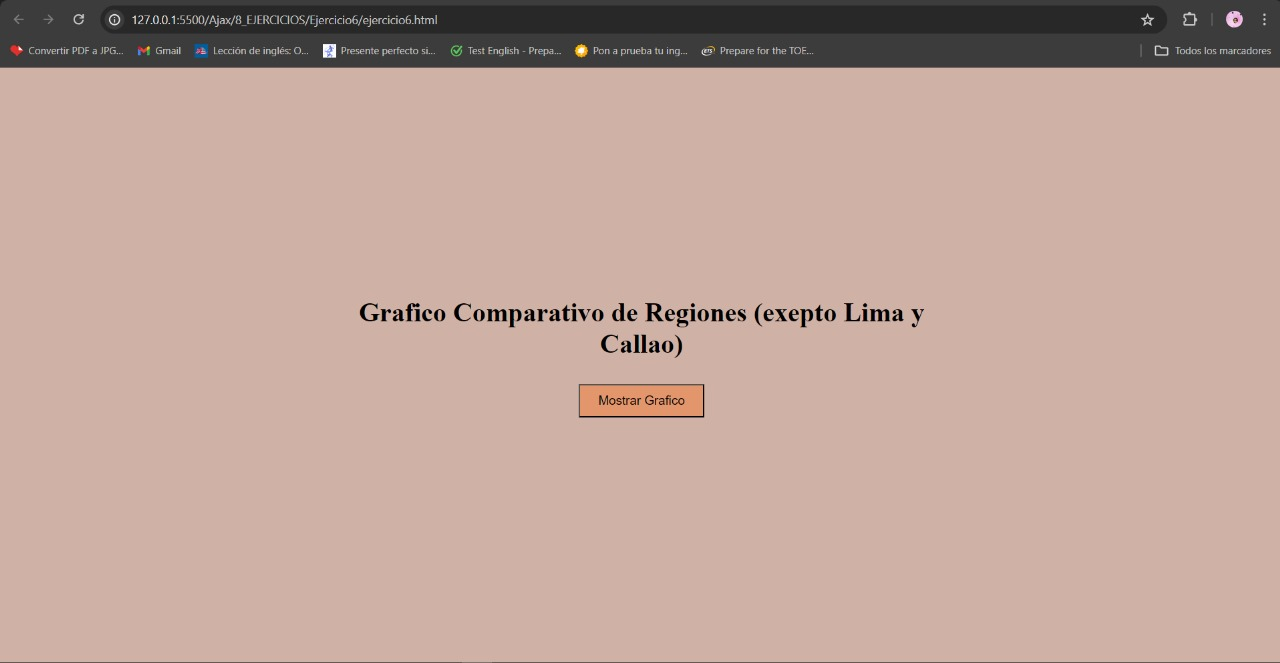
\includegraphics[width=1.0\textwidth,keepaspectratio]{img/Ejer6T2Pagina.jpg}
			%\includesvg{img/automata.svg}
			%\label{img:mot2}
			%\caption{Product backlog.}
		\end{figure}
		\item Resultado
		\begin{figure}[H]
			\centering
			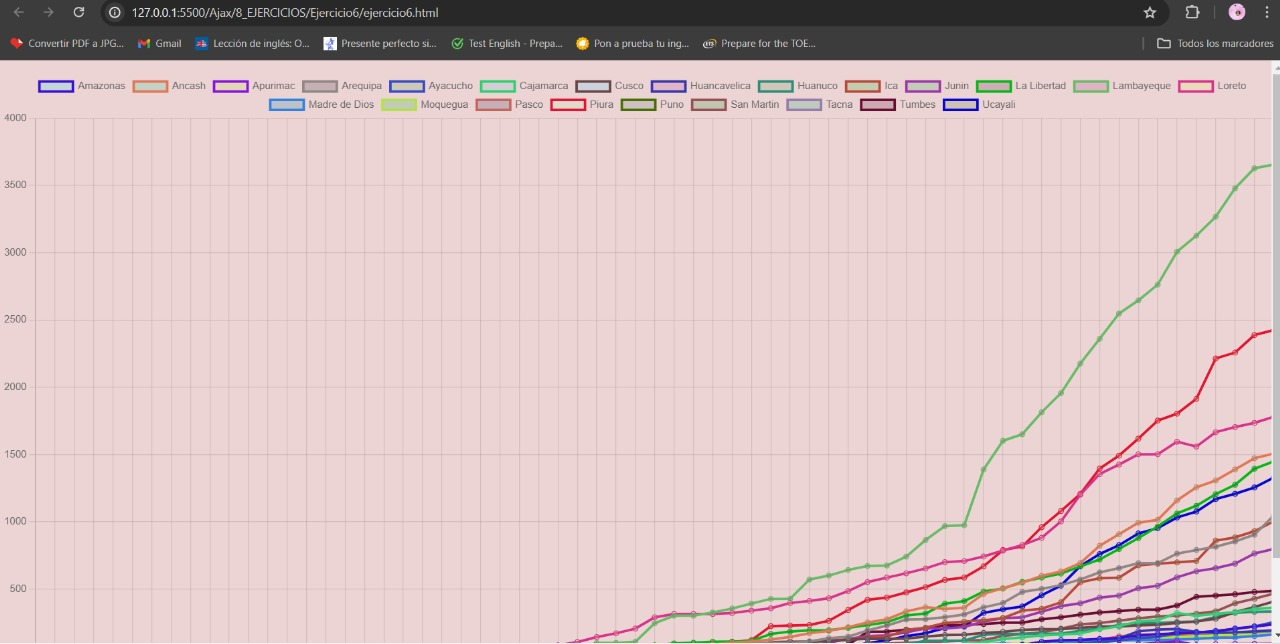
\includegraphics[width=1.0\textwidth,keepaspectratio]{img/Ejer6T2Result.jpg}
			%\includesvg{img/automata.svg}
			%\label{img:mot2}
			%\caption{Product backlog.}
		\end{figure}
	\end{itemize}
	
	\subsection{Haga gráficos comparativos entre regiones elegidas por el usuario.}
	
	\begin{itemize}
		\item HTML
		\begin{figure}[H]
			\centering
			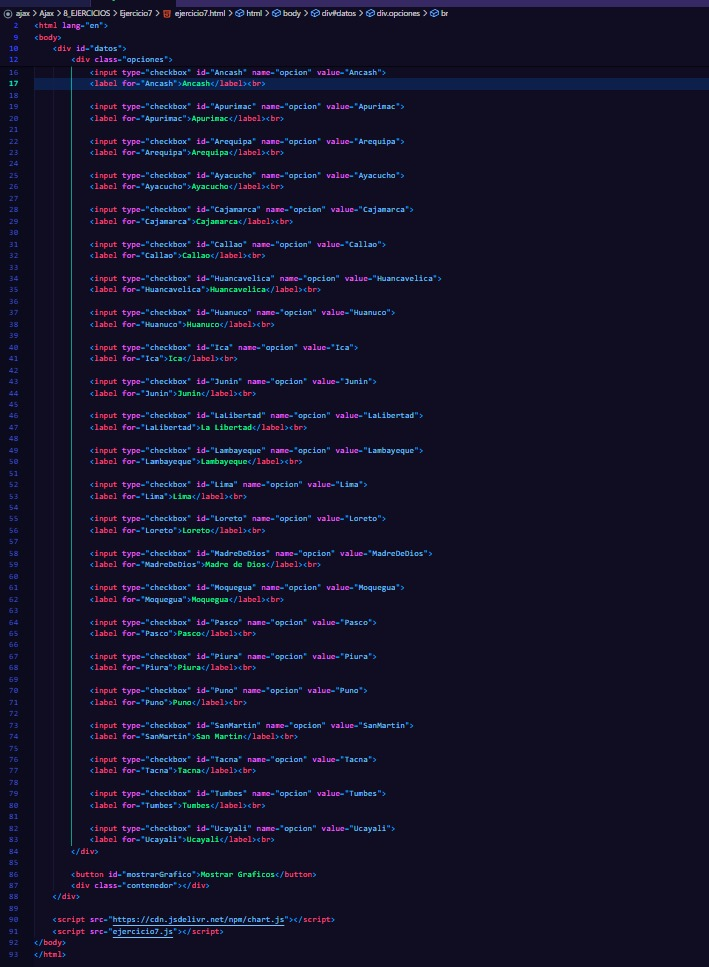
\includegraphics[width=1.0\textwidth,keepaspectratio]{img/Ejer7T2HTML.jpg}
			%\includesvg{img/automata.svg}
			%\label{img:mot2}
			%\caption{Product backlog.}
		\end{figure}
		\item Script
		\begin{figure}[H]
			\centering
			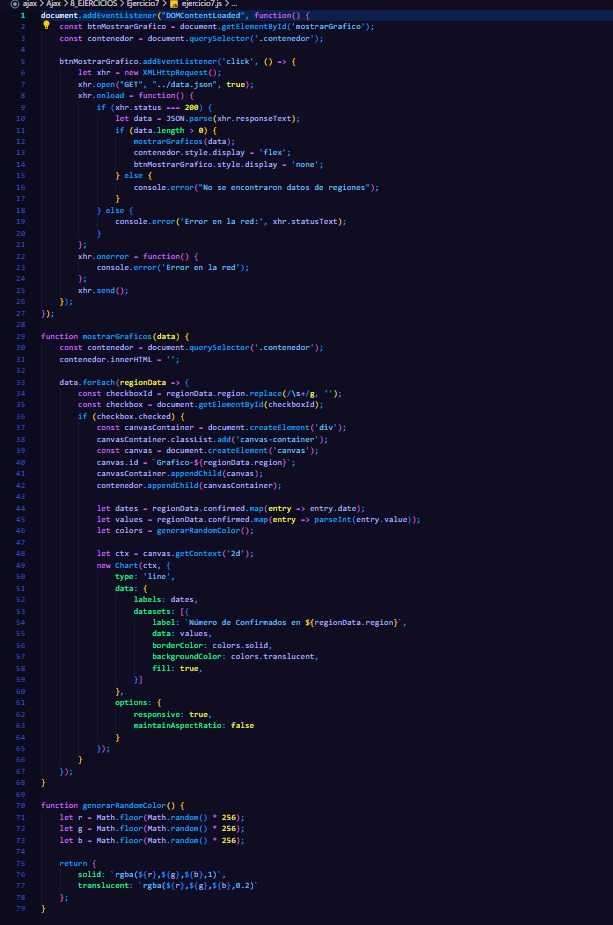
\includegraphics[width=1.0\textwidth,keepaspectratio]{img/Ejer7T2Script.jpg}
			%\includesvg{img/automata.svg}
			%\label{img:mot2}
			%\caption{Product backlog.}
		\end{figure}
		\item Página
		\begin{figure}[H]
			\centering
			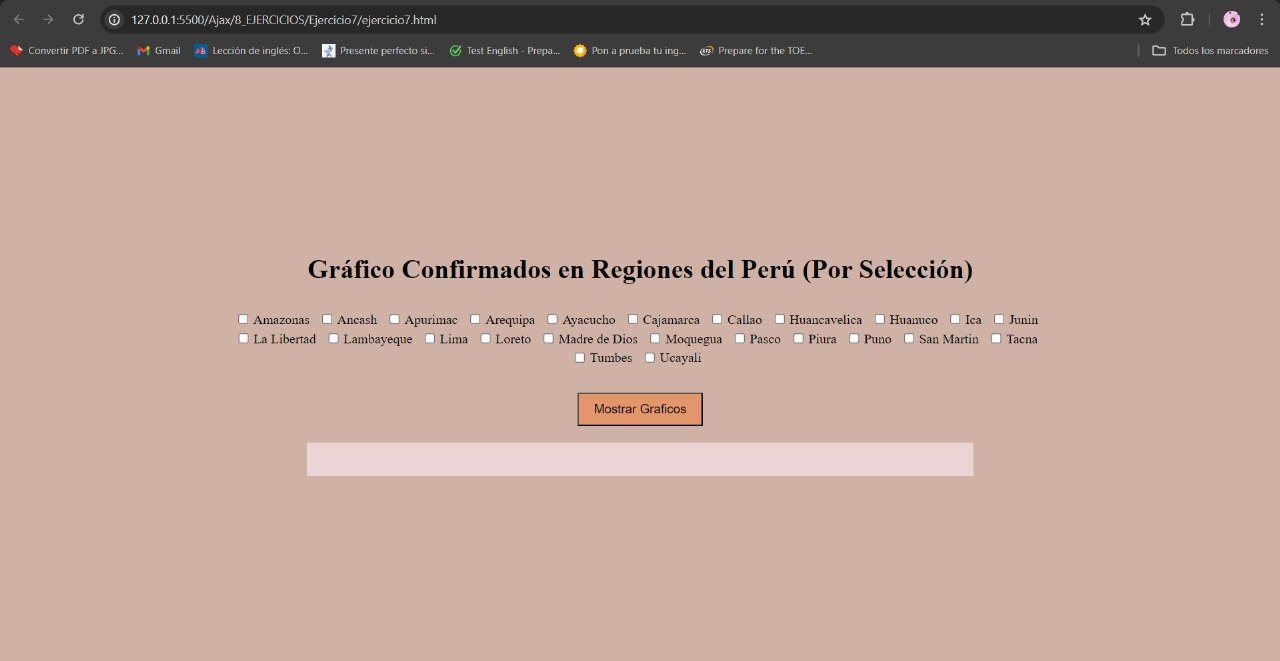
\includegraphics[width=1.0\textwidth,keepaspectratio]{img/Ejer7T2Pagina.jpg}
			%\includesvg{img/automata.svg}
			%\label{img:mot2}
			%\caption{Product backlog.}
		\end{figure}
		\item Resultado
		\begin{figure}[H]
			\centering
			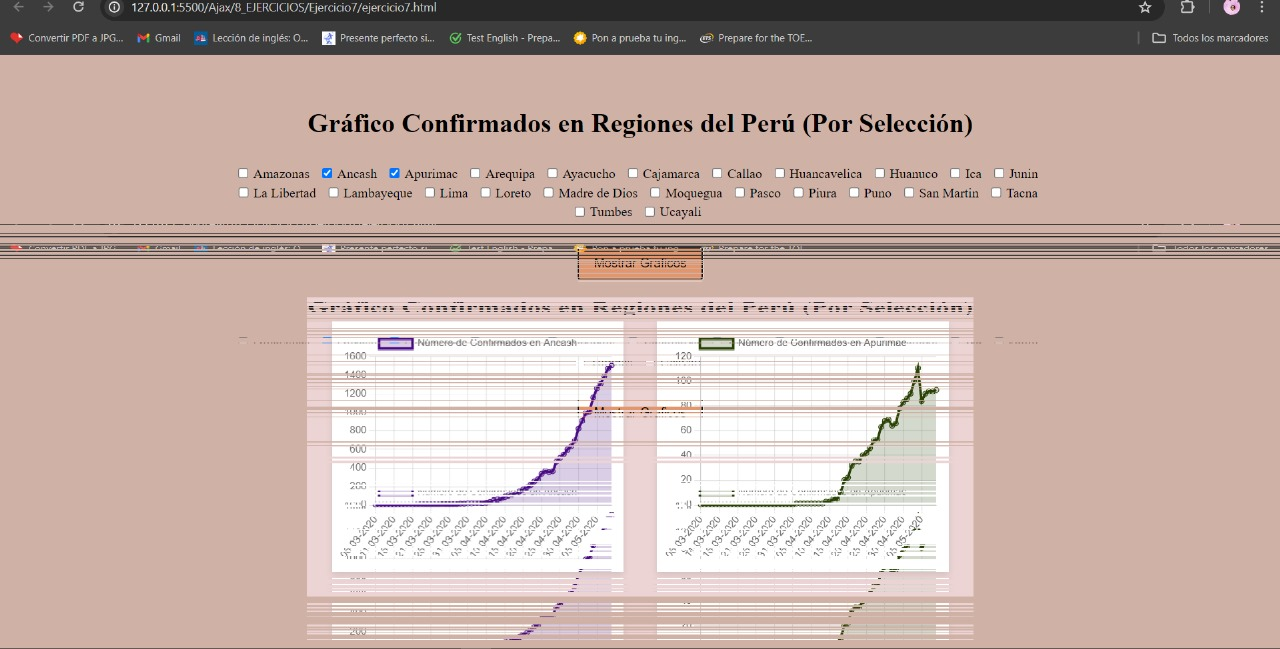
\includegraphics[width=1.0\textwidth,keepaspectratio]{img/Ejer7T2Result.jpg}
			%\includesvg{img/automata.svg}
			%\label{img:mot2}
			%\caption{Product backlog.}
		\end{figure}
	\end{itemize}
	
	\subsection{Visualice un gráfico comparativo del crecimiento en regiones excepto Lima y Callao, mostrando el número de confirmados por cada día}
	
	\begin{itemize}
		\item HTML
		\begin{figure}[H]
			\centering
			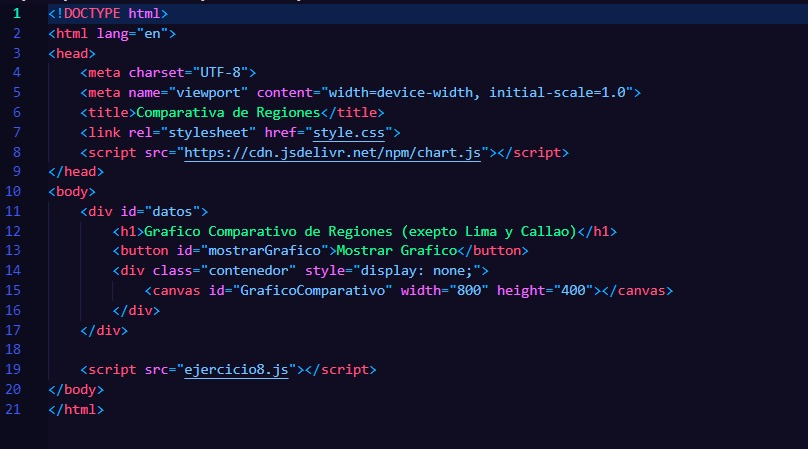
\includegraphics[width=1.0\textwidth,keepaspectratio]{img/Ejer8T2HTMl.jpg}
			%\includesvg{img/automata.svg}
			%\label{img:mot2}
			%\caption{Product backlog.}
		\end{figure}
		\item Script
		\begin{figure}[H]
			\centering
			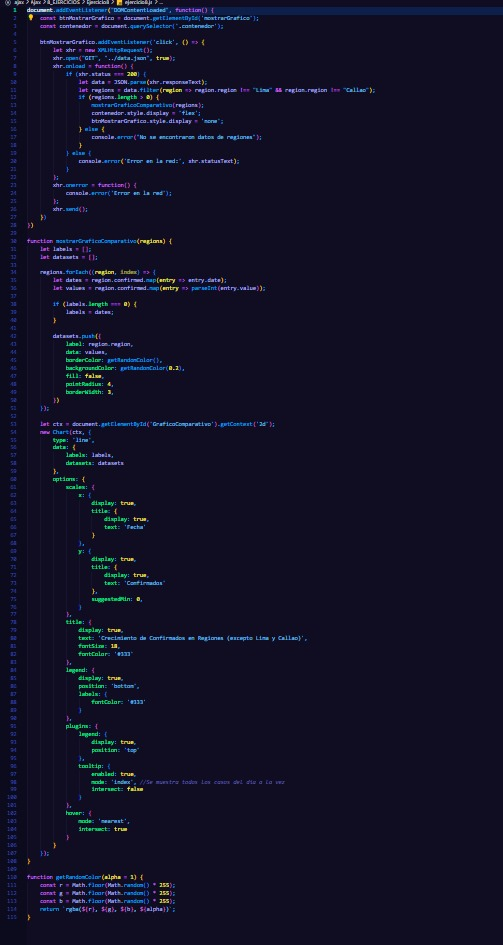
\includegraphics[width=1.0\textwidth,keepaspectratio]{img/Ejer8T2Script.jpg}
			%\includesvg{img/automata.svg}
			%\label{img:mot2}
			%\caption{Product backlog.}
		\end{figure}
		\item Página
		\begin{figure}[H]
			\centering
			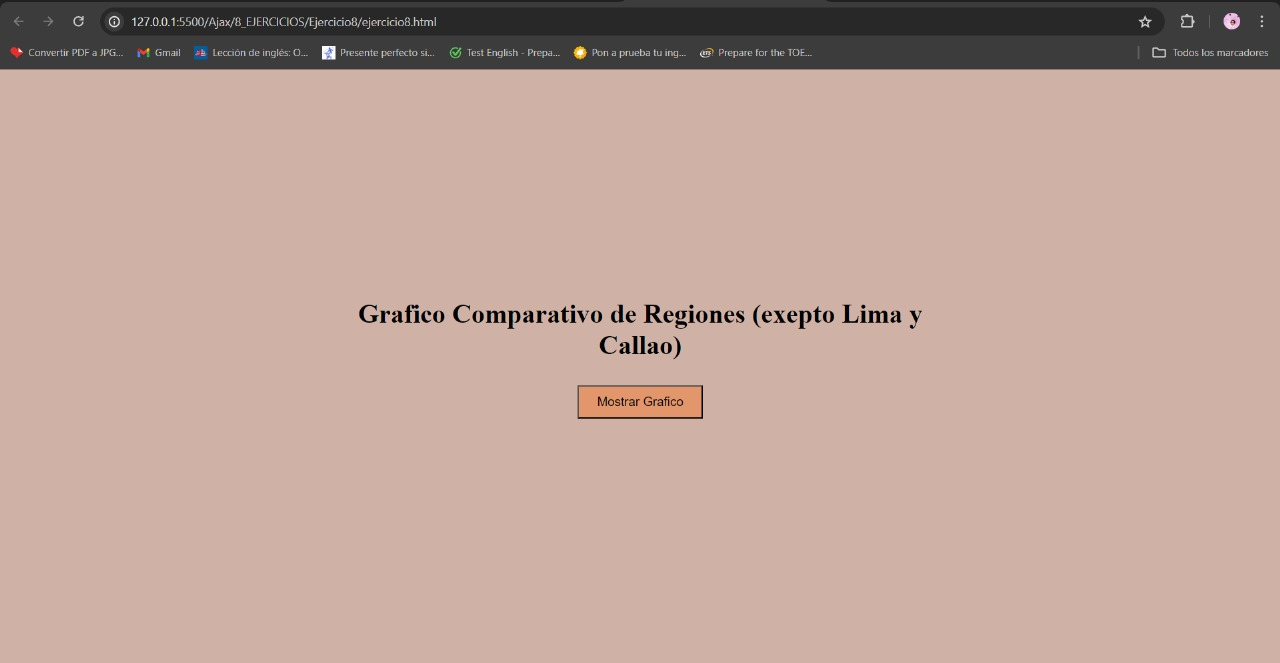
\includegraphics[width=1.0\textwidth,keepaspectratio]{img/Ejer8T2Pagina.jpg}
			%\includesvg{img/automata.svg}
			%\label{img:mot2}
			%\caption{Product backlog.}
		\end{figure}
		\item Resultado
		\begin{figure}[H]
			\centering
			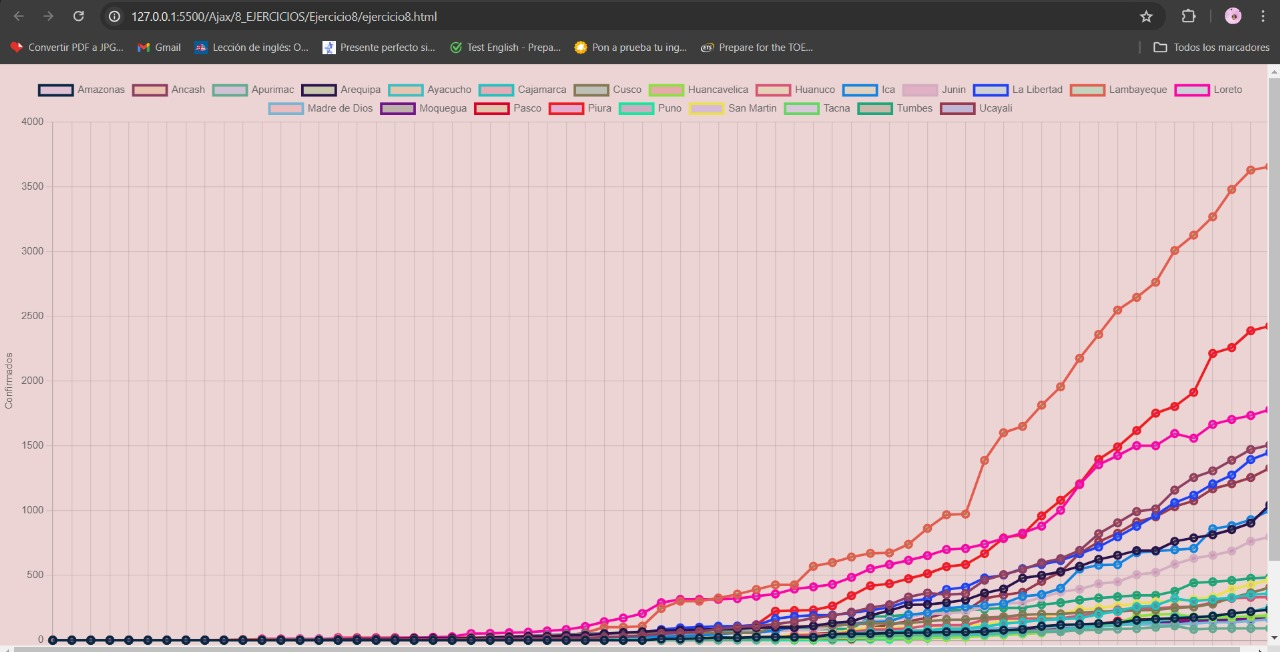
\includegraphics[width=1.0\textwidth,keepaspectratio]{img/Ejer8T2Result.jpg}
			%\includesvg{img/automata.svg}
			%\label{img:mot2}
			%\caption{Product backlog.}
		\end{figure}
	\end{itemize}

	%Section ws
	\section{w3schools}

	\subsection{Luis Guillermo Luque Condori}
	\subsubsection{Fotos de prueba}
	\begin{itemize}
		\item \begin{figure}[H]
			\centering
			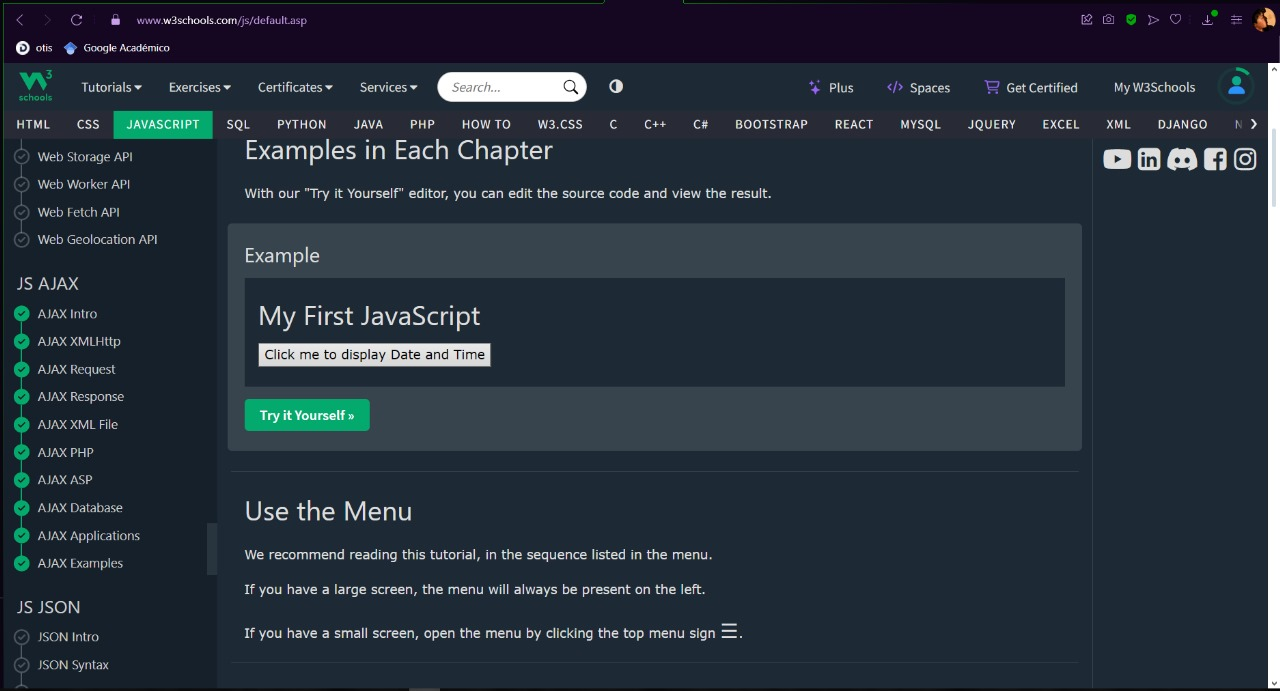
\includegraphics[width=1.0\textwidth,keepaspectratio]{img/wsLuis.jpg}
			%\includesvg{img/automata.svg}
			%\label{img:mot2}
			%\caption{Product backlog.}
		\end{figure}

		\begin{figure}[H]
			\centering
			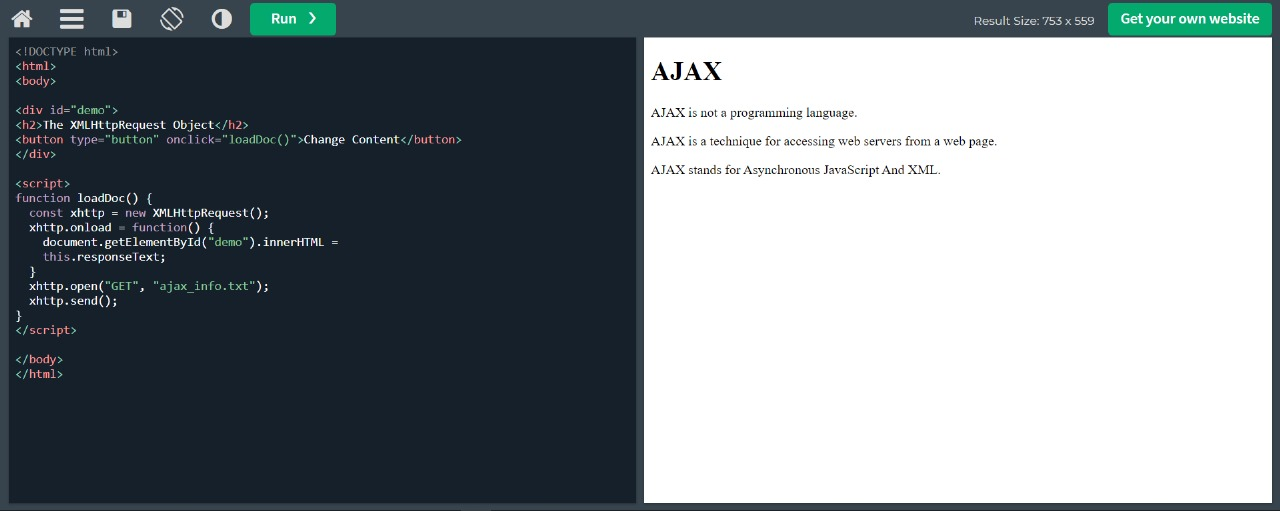
\includegraphics[width=1.0\textwidth,keepaspectratio]{img/L1.jpg}
			%\includesvg{img/automata.svg}
			%\label{img:mot2}
			%\caption{Product backlog.}
		\end{figure}
		\begin{figure}[H]
			\centering
			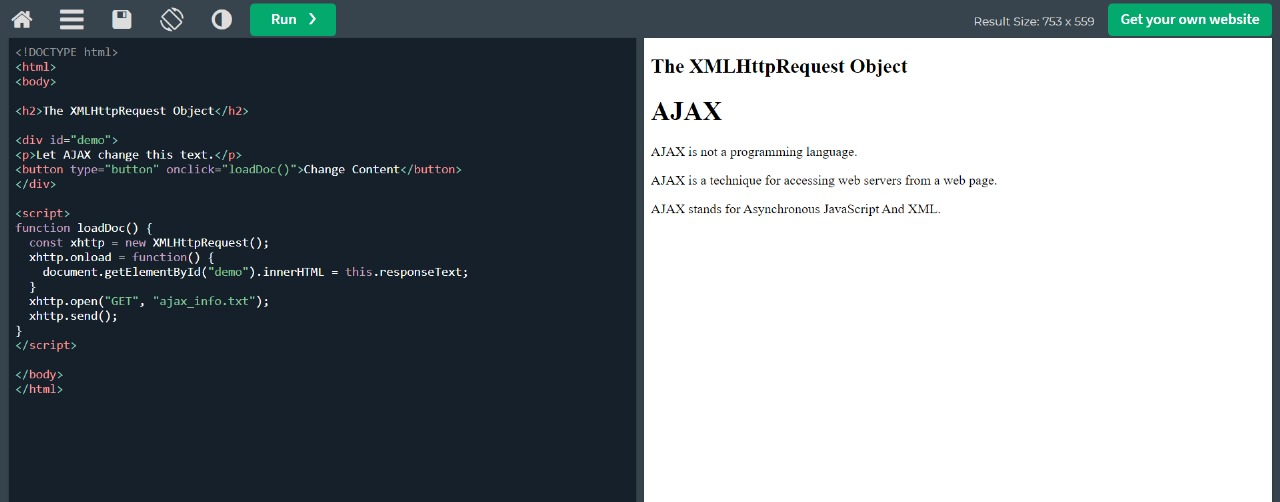
\includegraphics[width=1.0\textwidth,keepaspectratio]{img/L2.jpg}
			%\includesvg{img/automata.svg}
			%\label{img:mot2}
			%\caption{Product backlog.}
		\end{figure}
		\begin{figure}[H]
			\centering
			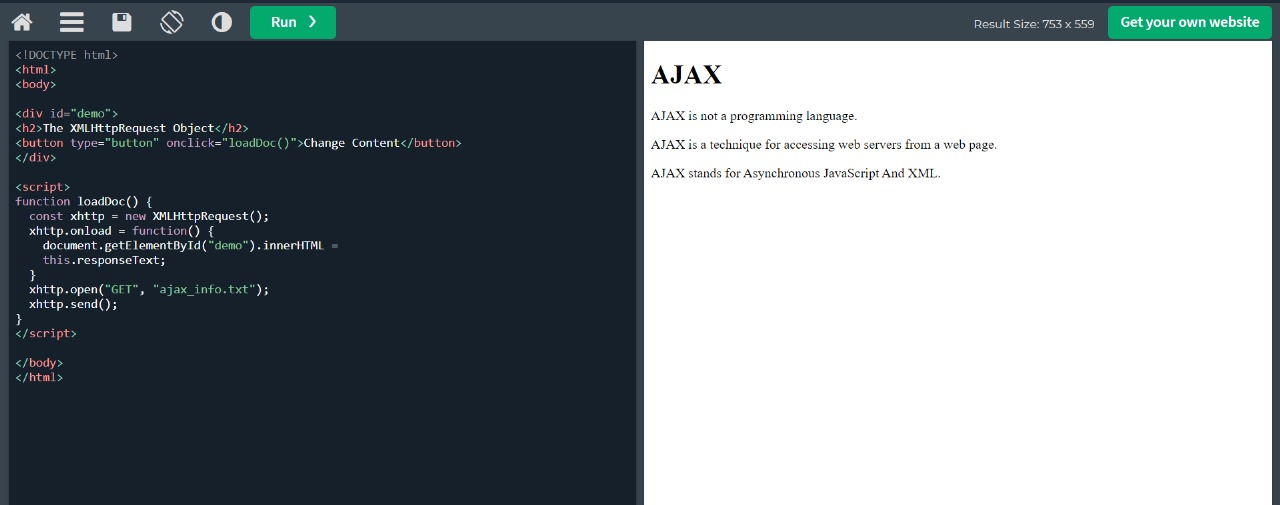
\includegraphics[width=1.0\textwidth,keepaspectratio]{img/L3.jpg}
			%\includesvg{img/automata.svg}
			%\label{img:mot2}
			%\caption{Product backlog.}
		\end{figure}
		\begin{figure}[H]
			\centering
			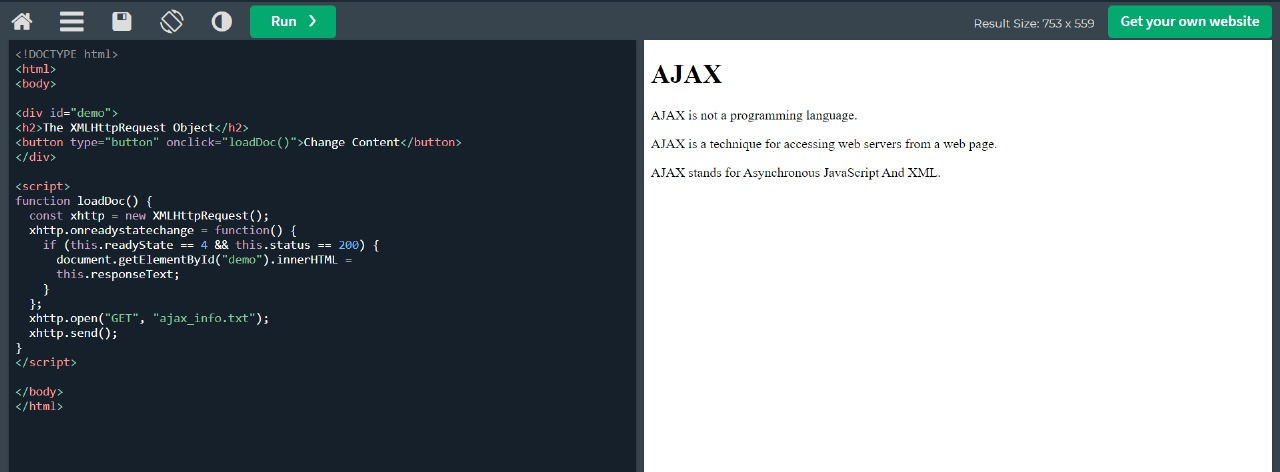
\includegraphics[width=1.0\textwidth,keepaspectratio]{img/L4.jpg}
			%\includesvg{img/automata.svg}
			%\label{img:mot2}
			%\caption{Product backlog.}
		\end{figure}
		\begin{figure}[H]
			\centering
			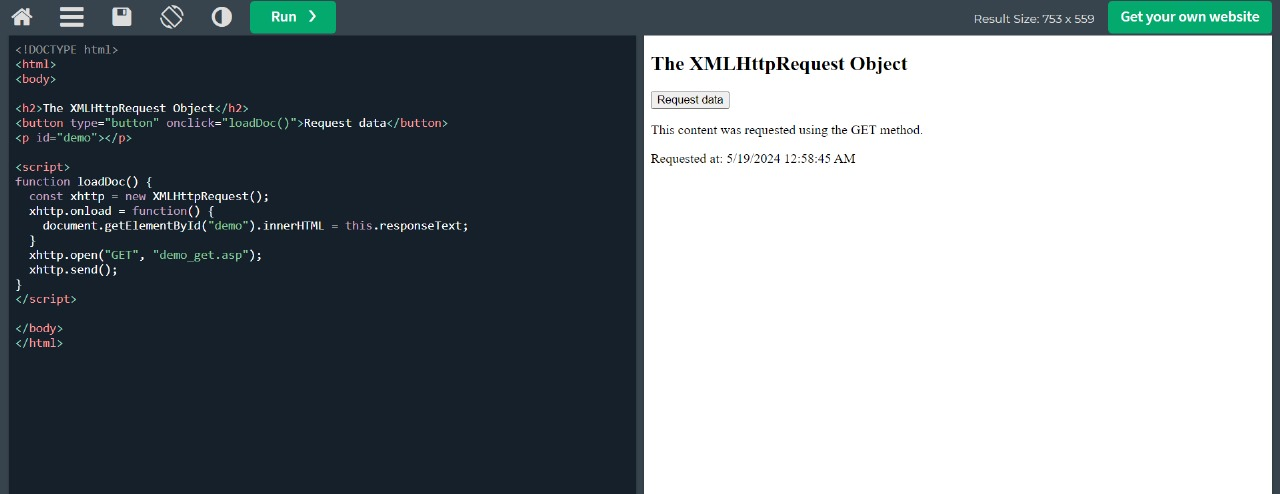
\includegraphics[width=1.0\textwidth,keepaspectratio]{img/L5.jpg}
			%\includesvg{img/automata.svg}
			%\label{img:mot2}
			%\caption{Product backlog.}
		\end{figure}
		\begin{figure}[H]
			\centering
			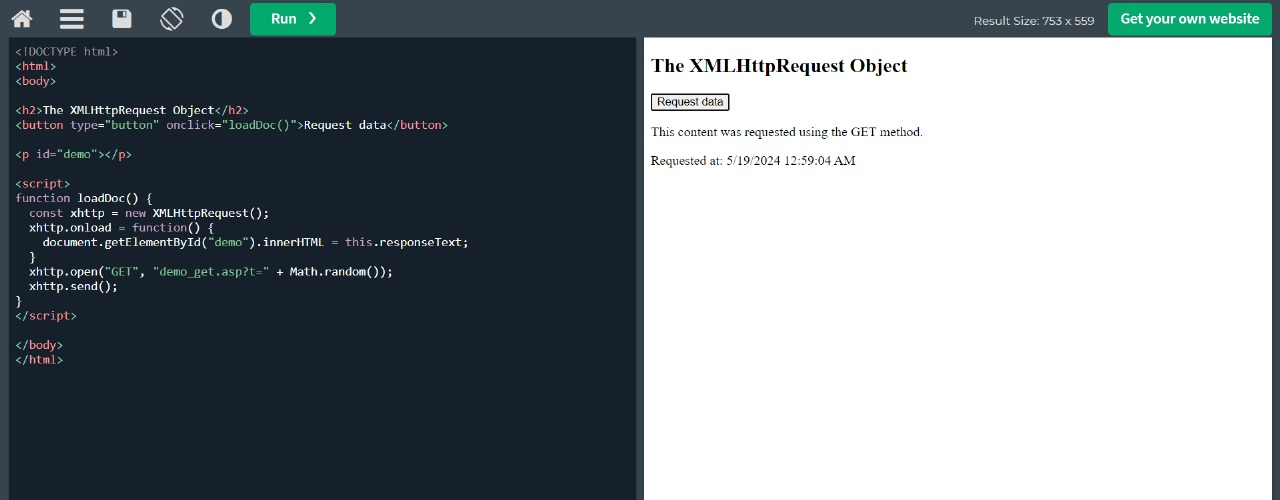
\includegraphics[width=1.0\textwidth,keepaspectratio]{img/L6.jpg}
			%\includesvg{img/automata.svg}
			%\label{img:mot2}
			%\caption{Product backlog.}
		\end{figure}
		\begin{figure}[H]
			\centering
			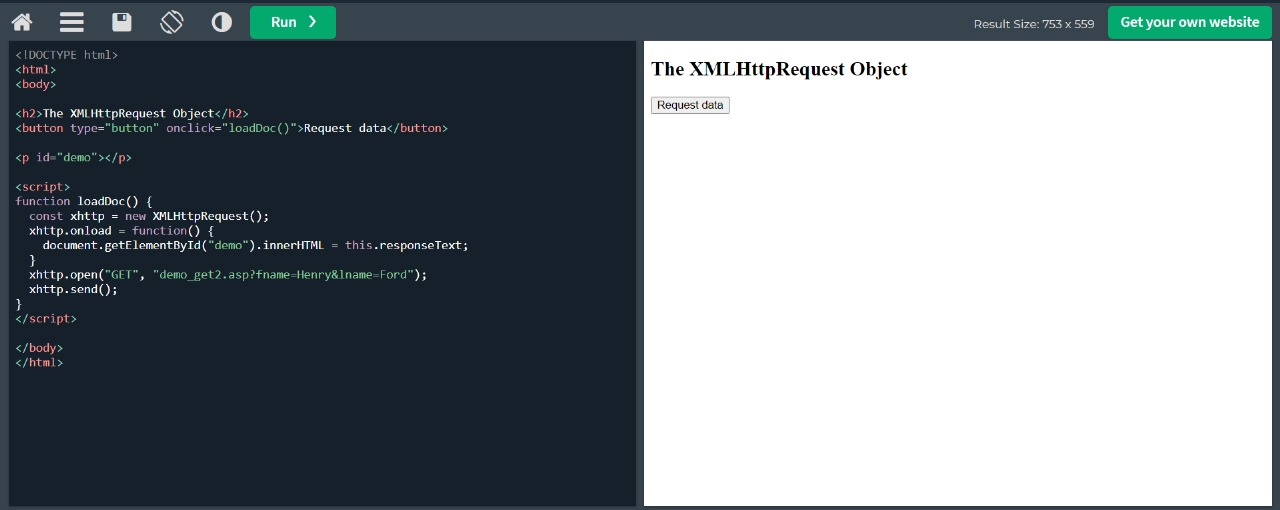
\includegraphics[width=1.0\textwidth,keepaspectratio]{img/L7.jpg}
			%\includesvg{img/automata.svg}
			%\label{img:mot2}
			%\caption{Product backlog.}
		\end{figure}
		\begin{figure}[H]
			\centering
			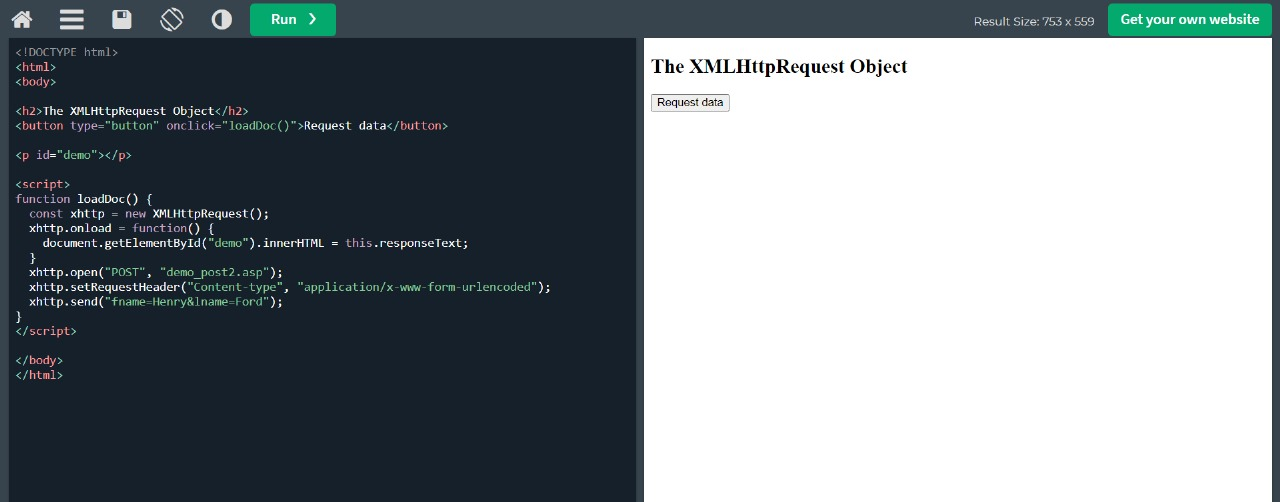
\includegraphics[width=1.0\textwidth,keepaspectratio]{img/L8.jpg}
			%\includesvg{img/automata.svg}
			%\label{img:mot2}
			%\caption{Product backlog.}
		\end{figure}
		\begin{figure}[H]
			\centering
			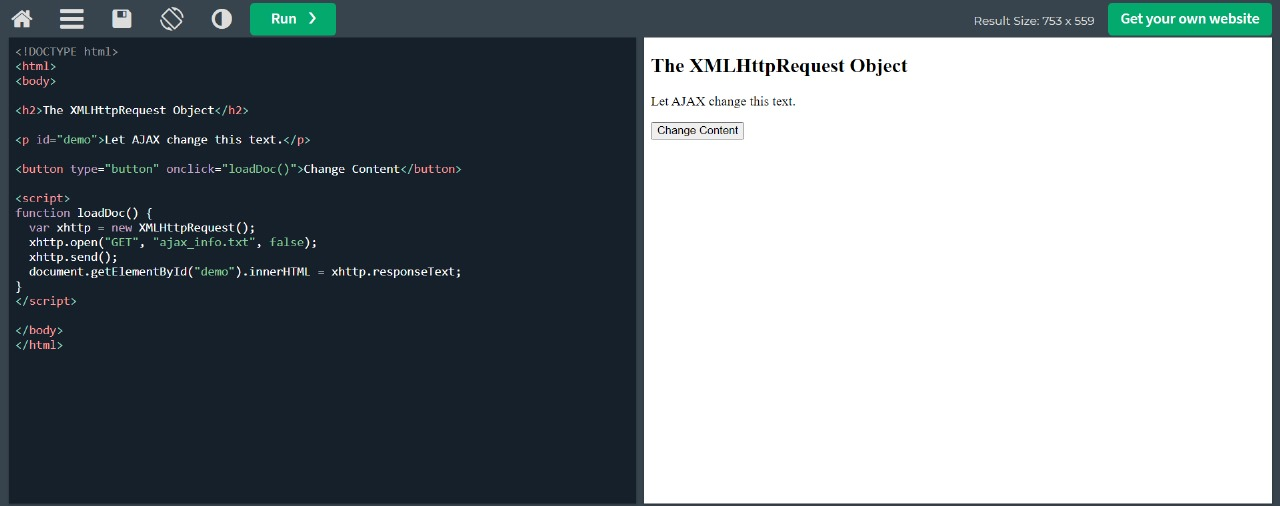
\includegraphics[width=1.0\textwidth,keepaspectratio]{img/L9.jpg}
			%\includesvg{img/automata.svg}
			%\label{img:mot2}
			%\caption{Product backlog.}
		\end{figure}
		\begin{figure}[H]
			\centering
			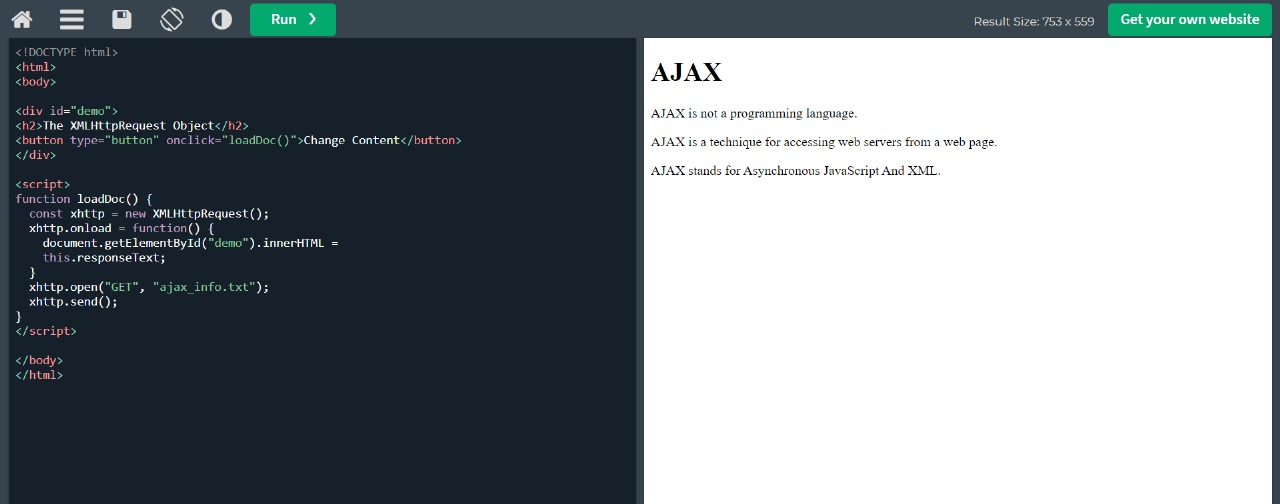
\includegraphics[width=1.0\textwidth,keepaspectratio]{img/L10.jpg}
			%\includesvg{img/automata.svg}
			%\label{img:mot2}
			%\caption{Product backlog.}
		\end{figure}
		\begin{figure}[H]
			\centering
			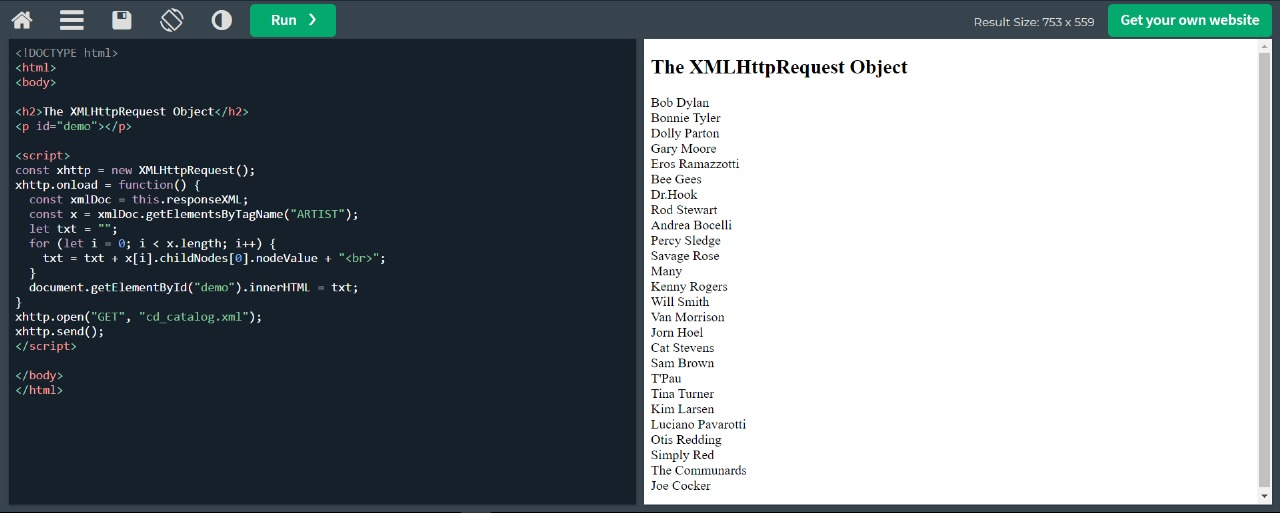
\includegraphics[width=1.0\textwidth,keepaspectratio]{img/L11.jpg}
			%\includesvg{img/automata.svg}
			%\label{img:mot2}
			%\caption{Product backlog.}
		\end{figure}
		\begin{figure}[H]
			\centering
			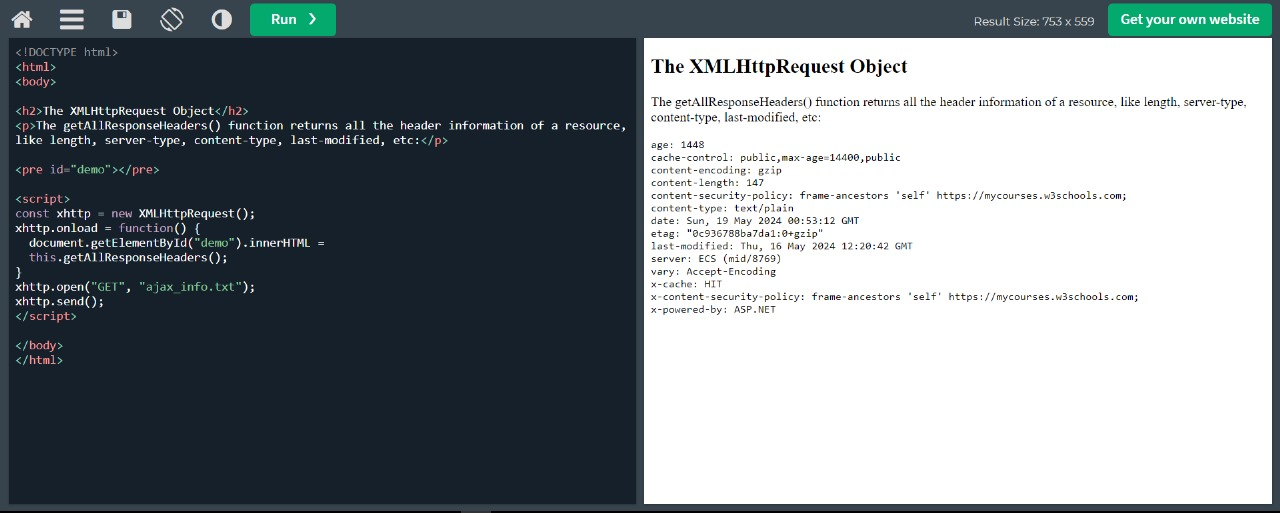
\includegraphics[width=1.0\textwidth,keepaspectratio]{img/L12.jpg}
			%\includesvg{img/automata.svg}
			%\label{img:mot2}
			%\caption{Product backlog.}
		\end{figure}
		\begin{figure}[H]
			\centering
			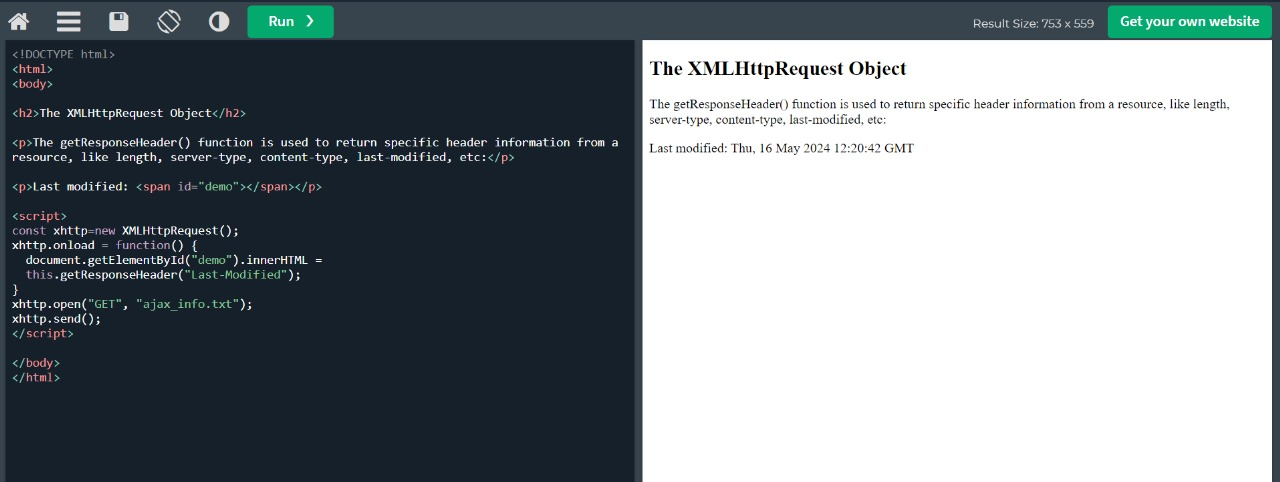
\includegraphics[width=1.0\textwidth,keepaspectratio]{img/L13.jpg}
			%\includesvg{img/automata.svg}
			%\label{img:mot2}
			%\caption{Product backlog.}
		\end{figure}
		\begin{figure}[H]
			\centering
			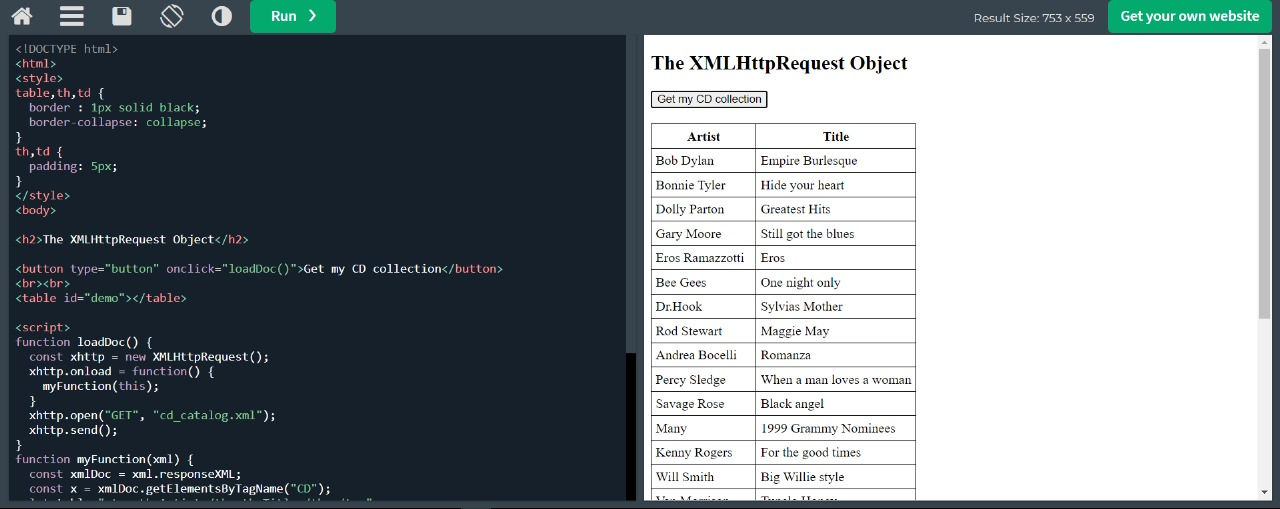
\includegraphics[width=1.0\textwidth,keepaspectratio]{img/L14.jpg}
			%\includesvg{img/automata.svg}
			%\label{img:mot2}
			%\caption{Product backlog.}
		\end{figure}
		\begin{figure}[H]
			\centering
			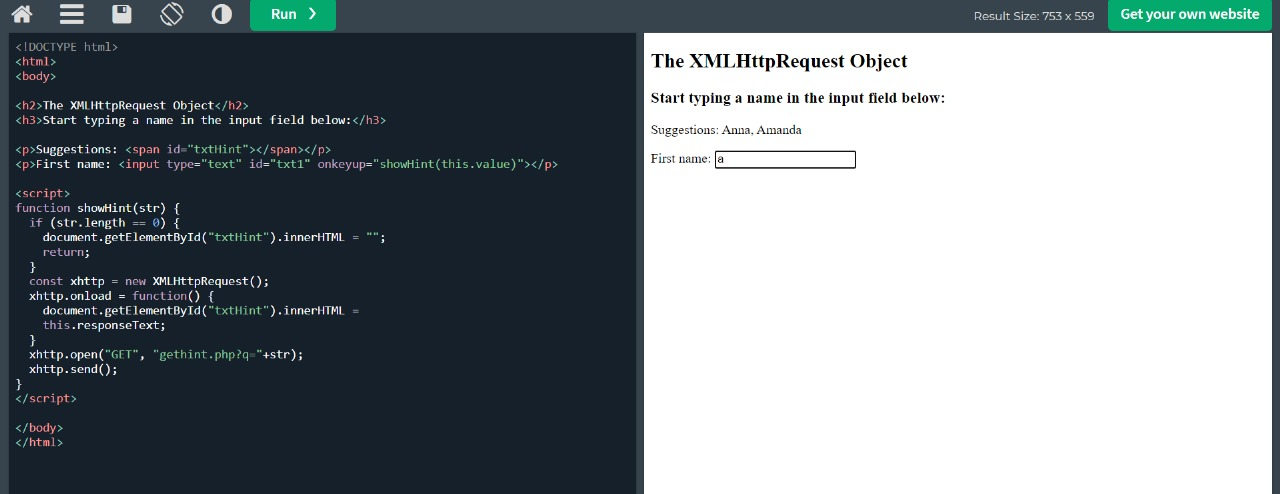
\includegraphics[width=1.0\textwidth,keepaspectratio]{img/L15.jpg}
			%\includesvg{img/automata.svg}
			%\label{img:mot2}
			%\caption{Product backlog.}
		\end{figure}
		\begin{figure}[H]
			\centering
			\includegraphics[width=1.0\textwidth,keepaspectratio]{img/L16.jpg}
			%\includesvg{img/automata.svg}
			%\label{img:mot2}
			%\caption{Product backlog.}
		\end{figure}
		\begin{figure}[H]
			\centering
			\includegraphics[width=1.0\textwidth,keepaspectratio]{img/L17.jpg}
			%\includesvg{img/automata.svg}
			%\label{img:mot2}
			%\caption{Product backlog.}
		\end{figure}		
	\end{itemize}
	
	\subsection{Fernando Miguel Garambel Marín}
	\subsubsection{Fotos de prueba}
	\begin{itemize}
		\item \begin{figure}[H]
			\centering
			\includegraphics[width=1.0\textwidth,keepaspectratio]{img/wsLuis.jpg}
			%\includesvg{img/automata.svg}
			%\label{img:mot2}
			%\caption{Product backlog.}
		\end{figure}
	\end{itemize}
	\subsection{William Herderson Choquehuanca Berma}
	\subsubsection{Fotos de prueba}
	\begin{itemize}
		\item \begin{figure}[H]
			\centering
			\includegraphics[width=1.0\textwidth,keepaspectratio]{img/wsLuis.jpg}
			%\includesvg{img/automata.svg}
			%\label{img:mot2}
			%\caption{Product backlog.}
		\end{figure}
	\end{itemize}
	\subsection{Jeans Anthony Ajra Huacso}
	\subsubsection{Fotos de prueba}
	\begin{itemize}
		\item \begin{figure}[H]
			\centering
			\includegraphics[width=1.0\textwidth,keepaspectratio]{img/A1.jpg}
			%\includesvg{img/automata.svg}
			%\label{img:mot2}
			%\caption{Product backlog.}
		\end{figure}

		\begin{figure}[H]
			\centering
			\includegraphics[width=1.0\textwidth,keepaspectratio]{img/A2.jpg}
			%\includesvg{img/automata.svg}
			%\label{img:mot2}
			%\caption{Product backlog.}
		\end{figure}

		\begin{figure}[H]
			\centering
			\includegraphics[width=1.0\textwidth,keepaspectratio]{img/A3.jpg}
			%\includesvg{img/automata.svg}
			%\label{img:mot2}
			%\caption{Product backlog.}
		\end{figure}

		\begin{figure}[H]
			\centering
			\includegraphics[width=1.0\textwidth,keepaspectratio]{img/A4.jpg}
			%\includesvg{img/automata.svg}
			%\label{img:mot2}
			%\caption{Product backlog.}
		\end{figure}

		\begin{figure}[H]
			\centering
			\includegraphics[width=1.0\textwidth,keepaspectratio]{img/A5.jpg}
			%\includesvg{img/automata.svg}
			%\label{img:mot2}
			%\caption{Product backlog.}
		\end{figure}

		\begin{figure}[H]
			\centering
			\includegraphics[width=1.0\textwidth,keepaspectratio]{img/A6.jpg}
			%\includesvg{img/automata.svg}
			%\label{img:mot2}
			%\caption{Product backlog.}
		\end{figure}

		\begin{figure}[H]
			\centering
			\includegraphics[width=1.0\textwidth,keepaspectratio]{img/A7.jpg}
			%\includesvg{img/automata.svg}
			%\label{img:mot2}
			%\caption{Product backlog.}
		\end{figure}

		\begin{figure}[H]
			\centering
			\includegraphics[width=1.0\textwidth,keepaspectratio]{img/A8.jpg}
			%\includesvg{img/automata.svg}
			%\label{img:mot2}
			%\caption{Product backlog.}
		\end{figure}

		\begin{figure}[H]
			\centering
			\includegraphics[width=1.0\textwidth,keepaspectratio]{img/A9.jpg}
			%\includesvg{img/automata.svg}
			%\label{img:mot2}
			%\caption{Product backlog.}
		\end{figure}

		\begin{figure}[H]
			\centering
			\includegraphics[width=1.0\textwidth,keepaspectratio]{img/A10.jpg}
			%\includesvg{img/automata.svg}
			%\label{img:mot2}
			%\caption{Product backlog.}
		\end{figure}


		\begin{figure}[H]
			\centering
			\includegraphics[width=1.0\textwidth,keepaspectratio]{img/A11.jpg}
			%\includesvg{img/automata.svg}
			%\label{img:mot2}
			%\caption{Product backlog.}
		\end{figure}
		\begin{figure}[H]
			\centering
			\includegraphics[width=1.0\textwidth,keepaspectratio]{img/A12.jpg}
			%\includesvg{img/automata.svg}
			%\label{img:mot2}
			%\caption{Product backlog.}
		\end{figure}

		\begin{figure}[H]
			\centering
			\includegraphics[width=1.0\textwidth,keepaspectratio]{img/A13.jpg}
			%\includesvg{img/automata.svg}
			%\label{img:mot2}
			%\caption{Product backlog.}
		\end{figure}


		\begin{figure}[H]
			\centering
			\includegraphics[width=1.0\textwidth,keepaspectratio]{img/A14.jpg}
			%\includesvg{img/automata.svg}
			%\label{img:mot2}
			%\caption{Product backlog.}
		\end{figure}

		\begin{figure}[H]
			\centering
			\includegraphics[width=1.0\textwidth,keepaspectratio]{img/A15.jpg}
			%\includesvg{img/automata.svg}
			%\label{img:mot2}
			%\caption{Product backlog.}
		\end{figure}
		\begin{figure}[H]
			\centering
			\includegraphics[width=1.0\textwidth,keepaspectratio]{img/A16.jpg}
			%\includesvg{img/automata.svg}
			%\label{img:mot2}
			%\caption{Product backlog.}
		\end{figure}
		\begin{figure}[H]
			\centering
			\includegraphics[width=1.0\textwidth,keepaspectratio]{img/A17.jpg}
			%\includesvg{img/automata.svg}
			%\label{img:mot2}
			%\caption{Product backlog.}
		\end{figure}
		\begin{figure}[H]
			\centering
			\includegraphics[width=1.0\textwidth,keepaspectratio]{img/A18.jpg}
			%\includesvg{img/automata.svg}
			%\label{img:mot2}
			%\caption{Product backlog.}
		\end{figure}
		\begin{figure}[H]
			\centering
			\includegraphics[width=1.0\textwidth,keepaspectratio]{img/A19.jpg}
			%\includesvg{img/automata.svg}
			%\label{img:mot2}
			%\caption{Product backlog.}
		\end{figure}
		\begin{figure}[H]
			\centering
			\includegraphics[width=1.0\textwidth,keepaspectratio]{img/A20.jpg}
			%\includesvg{img/automata.svg}
			%\label{img:mot2}
			%\caption{Product backlog.}
		\end{figure}

		\begin{figure}[H]
			\centering
			\includegraphics[width=1.0\textwidth,keepaspectratio]{img/A21.jpg}
			%\includesvg{img/automata.svg}
			%\label{img:mot2}
			%\caption{Product backlog.}
		\end{figure}

	\end{itemize}







\clearpage

	\section{\textcolor{red}{Rúbricas}}
	
	\subsection{\textcolor{red}{Entregable Informe}}
	\begin{table}[H]
		\caption{Tipo de Informe}
		\setlength{\tabcolsep}{0.5em} % for the horizontal padding
		{\renewcommand{\arraystretch}{1.5}% for the vertical padding
		\begin{tabular}{|p{3cm}|p{12cm}|}
			\hline
			\multicolumn{2}{|c|}{\textbf{\textcolor{red}{Informe}}}  \\
			\hline 
			\textbf{\textcolor{red}{Latex}} & \textcolor{blue}{El informe está en formato PDF desde Latex,  con un formato limpio (buena presentación) y facil de leer.}   \\ 
			\hline 
			
			
		\end{tabular}
	}
	\end{table}
	
	\clearpage
	
	\subsection{\textcolor{red}{Rúbrica para el contenido del Informe y demostración}}
	\begin{itemize}			
		\item El alumno debe marcar o dejar en blanco en celdas de la columna \textbf{Checklist} si cumplio con el ítem correspondiente.
		\item Si un alumno supera la fecha de entrega,  su calificación será sobre la nota mínima aprobada, siempre y cuando cumpla con todos lo items.
		\item El alumno debe autocalificarse en la columna \textbf{Estudiante} de acuerdo a la siguiente tabla:
	
		\begin{table}[ht]
			\caption{Niveles de desempeño}
			\begin{center}
			\begin{tabular}{ccccc}
    			\hline
    			 & \multicolumn{4}{c}{Nivel}\\
    			\cline{1-5}
    			\textbf{Puntos} & Insatisfactorio 25\%& En Proceso 50\% & Satisfactorio 75\% & Sobresaliente 100\%\\
    			\textbf{2.0}&0.5&1.0&1.5&2.0\\
    			\textbf{4.0}&1.0&2.0&3.0&4.0\\
    		\hline
			\end{tabular}
		\end{center}
	\end{table}	
	
	\end{itemize}
	
	\begin{table}[H]
		\caption{Rúbrica para contenido del Informe y demostración}
		\setlength{\tabcolsep}{0.5em} % for the horizontal padding
		{\renewcommand{\arraystretch}{1.5}% for the vertical padding
		%\begin{center}
		\begin{tabular}{|p{2.7cm}|p{7cm}|x{1.3cm}|p{1.2cm}|p{1.5cm}|p{1.1cm}|}
			\hline
    		\multicolumn{2}{|c|}{Contenido y demostración} & Puntos & Checklist & Estudiante & Profesor\\
			\hline
			\textbf{1. GitHub} & Hay enlace URL activo del directorio para el  laboratorio hacia su repositorio GitHub con código fuente terminado y fácil de revisar. &2 &X &2 & \\ 
			\hline
			\textbf{2. Commits} &  Hay capturas de pantalla de los commits más importantes con sus explicaciones detalladas. (El profesor puede preguntar para refrendar calificación). &4 &X &2 & \\ 
			\hline 
			\textbf{3. Código fuente} &  Hay porciones de código fuente importantes con numeración y explicaciones detalladas de sus funciones. &2 &X &1 & \\ 
			\hline 
			\textbf{4. Ejecución} & Se incluyen ejecuciones/pruebas del código fuente  explicadas gradualmente. &2 &X &2 & \\ 
			\hline			
			\textbf{5. Pregunta} & Se responde con completitud a la pregunta formulada en la tarea.  (El profesor puede preguntar para refrendar calificación).  &2 &X &2 & \\ 
			\hline	
			\textbf{6. Fechas} & Las fechas de modificación del código fuente estan dentro de los plazos de fecha de entrega establecidos. &2 &X &2 & \\ 
			\hline 
			\textbf{7. Ortografía} & El documento no muestra errores ortográficos. &2 &X &1 & \\ 
			\hline 
			\textbf{8. Madurez} & El Informe muestra de manera general una evolución de la madurez del código fuente,  explicaciones puntuales pero precisas y un acabado impecable.   (El profesor puede preguntar para refrendar calificación).  &4 &X &1 & \\ 
			\hline
			\multicolumn{2}{|c|}{\textbf{Total}} &20 & &13 & \\ 
			\hline
		\end{tabular}
		%\end{center}
		%\label{tab:multicol}
		}
	\end{table}
	
\clearpage

\section{Referencias}
\begin{itemize}			
	\item \url{https://www.w3schools.com/java/default.asp}
	\item \url{https://www.geeksforgeeks.org/insertion-sort/}
\end{itemize}	
	
%\clearpage
%\bibliographystyle{apalike}
%\bibliographystyle{IEEEtranN}
%\bibliography{bibliography}

\end{document}